\documentclass[t, aspectratio=169]{beamer}

\usepackage[english]{babel}
\usepackage[utf8]{inputenc}
\usepackage{amsthm}
\usepackage{amsmath}
\usepackage{amsfonts}
\usepackage{graphicx}
\usepackage{tikz} % for diagrams
\usetikzlibrary[positioning]
\usetikzlibrary[fit]
\usetikzlibrary{patterns}
\usetikzlibrary{patterns.meta}
\usetikzlibrary{shapes.geometric}
\usetikzlibrary{shapes.arrows}
\usetikzlibrary{shapes}
\usetikzlibrary{arrows.meta}
\usetikzlibrary{calc}
\usetikzlibrary{tikzmark}
\usetikzlibrary{datavisualization}
\usetikzlibrary{datavisualization.formats.functions}
\usetikzlibrary{tikzmark}
%\usetikzlibrary{uml}
%\usepackage{tikz-uml} % https://perso.ensta-paris.fr/~kielbasi/tikzuml/index.php
\usepackage{pgf-umlcd}
\usepackage{pgfplots} % for plotting
\usepackage{adjustbox}
\usepackage{graphics}
\usepackage{tikz}
\usepackage{hyperref}
\usepackage{xspace} % for xspace
\usepackage{color} % for colored text
\usepackage{color, colortbl} % for colored tables
\usepackage{xcolor} % for colored cells in tables
\usepackage{fancyvrb} % for different fontsize in verbatim
\usepackage[T1]{fontenc} % for |
\usepackage{qrcode} % for QR codes
\usepackage{verbatim} % for verbatiminput
\usepackage{multicol} % for multicols
\usepackage{multirow} % for multirow
\usepackage{ragged2e} % for flushright environment
\usepackage{mathtools} % for mathmakebox
\usepackage{array} % for new array implementation: http://mirrors.ibiblio.org/CTAN/macros/latex/required/tools/array.pdf
\usepackage{dirtytalk} % for \say quotation
\usepackage{MnSymbol,wasysym} % for smileys
%\usepackage{enumitem} % for ordered and unordered list
\usepackage{longtable} % for tabular environment that spans multiple pages and supports footnotes

%\usepackage[danish]{babel} % load typographical rules for the english language
\usepackage{graphics} % for \scalebox
\usepackage{hyperref} % for \href
\usepackage{xcolor} % for text color
\usepackage{enumitem} % for ordered and unordered list
\usepackage{graphicx} % for images
\usepackage{pdfpages} % for including pdfs
\usepackage{footnote} % for footnotes
\usepackage{longtable} % for tabular environment that spans multiple pages and supports footnotes
\usepackage{colortbl} % for cell coloring
\usepackage{multirow} % for \multicolumn

% https://github.com/latex3/babel/issues/51
\makeatletter\AtBeginDocument{\let\@elt\relax}\makeatother

% styling
\setsecnumdepth{subsubsection} % how deep to number sections
\setlength{\parindent}{0em} % horizontal indent for first line of paragraph
\setlength{\parskip}{1em} % vertical space between paragraphs

\newcommand{\textdesc}[1]{\textit{\textbf{#1}}}
\newcommand{\descitem}[1]{\item \textdesc{#1}}

\title{\documenttitle\\\scalebox{0.85}{\documentsubtitle}}
\author{Aslak Johansen \href{mailto:asjo@mmmi.sdu.dk}{asjo@mmmi.sdu.dk}\\Aisha Umair \href{mailto:aiu@mmmi.sdu.dk}{aiu@mmmi.sdu.dk}}

\begin{document}

\maketitle
\setcounter{tocdepth}{2}
\tableofcontentswrapper


\setcounter{tocdepth}{4}
\setcounter{secnumdepth}{4}

\newcommand{\hlthing}[1]{\textcolor{orange}{#1}}
\newcommand{\hlcomment}[1]{\textcolor{blue}{#1}}
\newcommand{\hldata}[1]{\textcolor{teal}{#1}}

\newcommand{\quoted}[1]{\textsl{\say{#1}}}

% tikz configuration
\usetikzlibrary{arrows.meta, matrix, decorations.pathreplacing}
\usetikzlibrary{positioning}

\definecolor{aqua}{rgb}{0.878, 1.0, 1.0} % matches the default line highlight of minted

% sparql highlighting
\usepackage[cache=false]{minted}            % code inclusion
\newminted{sparql}{xleftmargin=1em,mathescape, numbersep=5pt, frame=lines, framesep=2mm, fontsize=\scriptsize, linenos}

\usepackage{pifont}%http://ctan.org/pkg/pifont
% http://tex.stackexchange.com/questions/42619/x-mark-to-match-checkmark
\newcommand{\cmark}{\text{\ding{51}}}
\newcommand{\xmark}{\text{\ding{55}}}
\newcommand{\change}{\text{\ding{46}}}

\newcommand{\valuename}[1]{\texttt{#1}}
\newcommand{\varname}[1]{\texttt{\textcolor{teal}{#1}}}
\newcommand{\typename}[1]{\texttt{\textcolor{purple}{#1}}}
\newcommand{\classname}[1]{\typename{#1}}
\newcommand{\interfacename}[1]{\typename{#1}}
\newcommand{\exceptionname}[1]{\classname{#1}}
\newcommand{\methodname}[1]{\texttt{\textcolor{blue}{#1}}}
\newcommand{\funcname}[1]{\methodname{#1}}
\newcommand{\packagename}[1]{\texttt{#1}}
\newcommand{\filename}[1]{\texttt{#1}}
\newcommand{\keywordname}[1]{\texttt{#1}}

\newcommand{\textdesc}[1]{\textit{\textbf{#1}}}
\newcommand{\descitem}[1]{\item \textdesc{#1}}
\newcommand{\includeSVG}[1]{
\includegraphics[scale=1.0]{./figs/#1.pdf}
}
\newcommand{\includeSVGfs}[1]{
\includegraphics[width=\paperwidth]{./figs/#1.pdf}
}
\newcommand{\includeBitmap}[2]{
\includegraphics[width=#2]{./figs/#1}
}

% args: 1:prefix 2:semester 3:index_west 4:index_east 5:title 6:ects 7:style
\newcommand{\entry}[7]{
  \node[
    rectangle,
    draw=purple,
    anchor=south west,
    align=center,
    minimum height=\cellheight,
    minimum width=(#4-#3)*\cellwidth+((#4-#3)-1)*\cellspacing,
    #7
  ]
  (#1) at (
    [
      xshift=\xoffset+#3*\cellwidth+(#3-1)*\cellspacing,
      yshift=\yoffset+(#2-1)*\cellheight+(#2-2)*\cellspacing,
    ] semorigo)
  {
    #5\\\textcolor{orange}{#6 ECTS}
  }
}

\newcommand{\entryNormal}[6]{\entry{#1}{#2}{#3}{#4}{#5}{#6}{}}
\newcommand{\entryProject}[6]{\entry{#1}{#2}{#3}{#4}{#5}{#6}{fill=purple!10,}}
\newcommand{\entryElective}[6]{\entry{#1}{#2}{#3}{#4}{#5}{#6}{pattern=north east lines, pattern color=purple!10, even odd rule,}}
\newcommand{\entryNormalMsc}[6]{\entry{#1}{#2}{#3}{#4}{#5}{#6}{draw=blue}}
\newcommand{\entryProjectMsc}[6]{\entry{#1}{#2}{#3}{#4}{#5}{#6}{draw=blue,fill=blue!10,}}
\newcommand{\entryElectiveMsc}[6]{\entry{#1}{#2}{#3}{#4}{#5}{#6}{draw=blue,pattern=north east lines, pattern color=blue!10, even odd rule,}}

\newenvironment{inspiration}[1]
{
    \begin{center}
    \newcommand{\temp}{#1}
    \begin{minipage}{0.9\textwidth}
}
{
    \\
    \raggedright{-- \temp}
    \end{minipage}
    \end{center}
}

%% bypass highlighting of syntax errors in minted
%\renewcommand{\fcolorbox}[4][]{#4}

% remove paragraph indent
\setlength{\parindent}{0in}

% remove footer
\setbeamertemplate{footline}[page number]{} % gets rid of bottom navigation bars
\setbeamertemplate{navigation symbols}{} % gets rid of navigation symbols
\usecolortheme{default}
\definecolor{structurecolor}{RGB}{21,66,129}
\setbeamercolor{structure}{fg=structurecolor}
\setbeamertemplate{footline}{}

% PDF settings
\hypersetup{
pdftitle={Software Engineering og Software Teknologi - Introduktion til Semesteret},
pdfauthor={Aslak Johansen, Aisha Umair},
pdfsubject={},
pdfkeywords={Software Engineering, Softwareteknologi, Semester}
}

\title{Software Engineering og Softwareteknologi \\ \scalebox{0.9}{Introduktion til Semesteret}}
\author{
Aslak Johansen \hspace{1mm} \href{mailto:asjo@mmmi.sdu.dk}{asjo@mmmi.sdu.dk} \\
Aisha Umair \hspace{1mm} \href{mailto:aiu@mmmi.sdu.dk}{aiu@mmmi.sdu.dk}
}
\logo{\vspace{-0.5mm}
\includegraphics[width=15mm]{figs/SDU.pdf}\hspace{0.5mm}}

\begin{document}

%%%%%%%%%%%%%%%%%%%%%%%%%%%%%%%%%%%%%%%%%%%%%%%%%%%%%%%%%%%%%%%
%%%%%%%%%%%%%%%%%%%%%%%%%%%%%%%%%%%%%%%%%%%%%%%%%%%%%%%%% Intro
\frame{\titlepage}
\logo{}

\section{Indhold}
\begin{frame}[fragile]
  \frametitle{Indhold}
  \vspace{2mm}
  \begin{columns}
    \begin{column}{0.55\textwidth}
      \begin{itemize}
        \item En syddansk ingeniør
        \item Første semester på Software Engineering og Softwareteknologi
        \item Semesterprojektet på 1. semester
        \item Problemorienteret projektarbejde
        \item Information om uddannelsesledelse og administration
        \item Introduktion til itslearning
        \item Online kursus i problemorienteret projektarbejde
        \item Afslutning
      \end{itemize}
    \end{column}
    \begin{column}{0.45\textwidth}
    \end{column}
  \end{columns}
  
  \begin{tikzpicture}[remember picture, overlay]
    \node[anchor=east] at ([xshift=1cm] current page.east) 
    {
        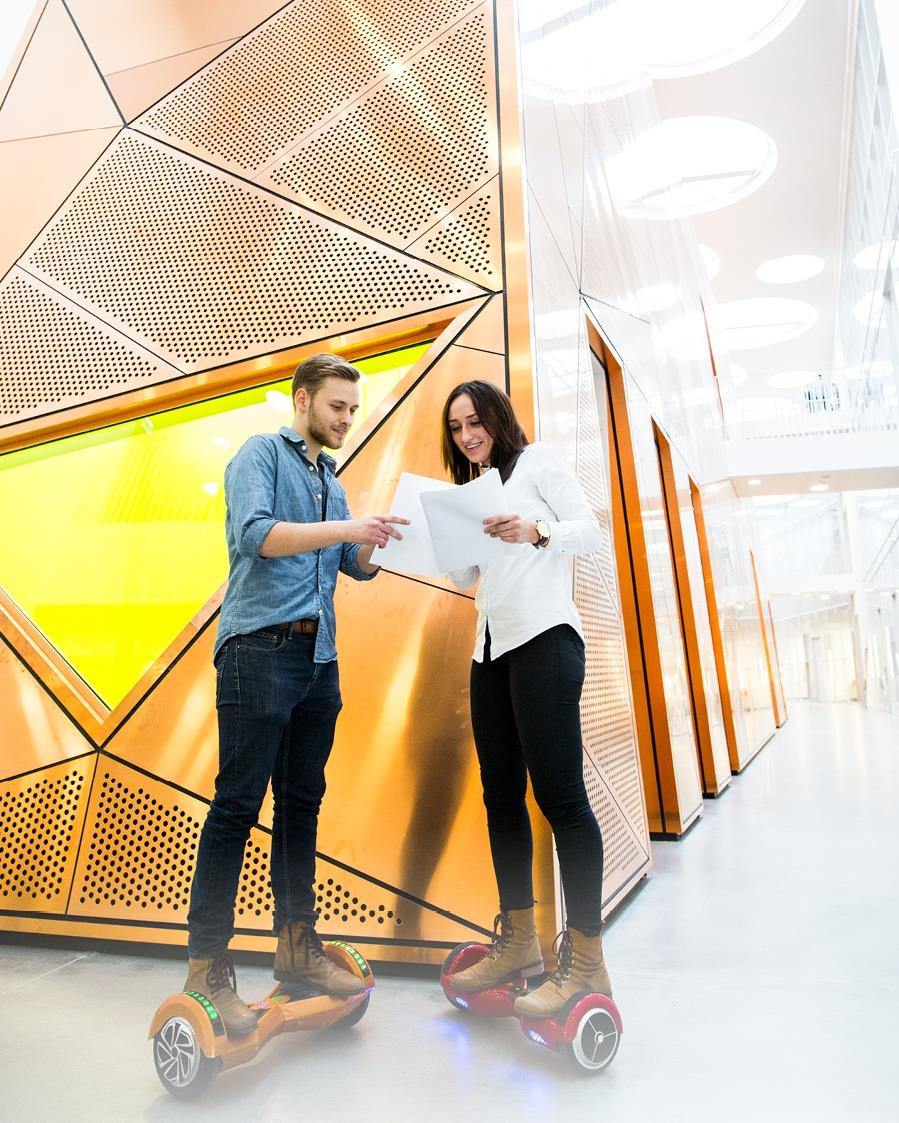
\includegraphics[height=\paperheight]{figs/image-001.png}
    };
  \end{tikzpicture}
\end{frame}

%%%%%%%%%%%%%%%%%%%%%%%%%%%%%%%%%%%%%%%%%%%%%%%%%%%%%%%%%%%%%%%
%%%%%%%%%%%%%%%%%%%%%%%%%%%%%%%%%%%%%%%% Den Syddanske Ingeniør
\section{Den Syddanske Ingeniør}
\begin{frame}
  \vspace{25mm}
  \begin{center}
    \Huge{Part 1:\\Den Syddanske Ingeniør}
  \end{center}
\end{frame}

\subsection{Hvad er en Ingeniør?}
\begin{frame}[fragile]
  \frametitle{Hvad er en Ingeniør?}
  
  \newcommand{\scaletext}[1]{\scriptsize{#1}}
  
  \vspace{0mm}
  \scaletext{
    Ingeniør, person, som er uddannet til at \only<1>{udføre teknisk forskning og udvikling samt til at løse tekniske opgaver}\only<2->{\textcolor{teal}{udføre teknisk forskning og udvikling samt til at løse tekniske opgaver}} og gennemføre projekter inden for bl.a. bygge- og anlægsarbejder, maskinkonstruktion, produktion og energi \only<-2>{under hensyntagen til mennesker, miljø og økonomi}\only<3->{\textcolor{teal}{under hensyntagen til mennesker, miljø og økonomi}}.
  }
  
  \vspace{3mm}
  \scaletext{
    \textbf{Etymologi:}
    Ordet ingeniør kommer af fransk ingénieur, afledt af mlat. ingenium '(krigs)maskine', af latin ingenium 'kløgt, begavelse, påfund'. 
  }
  
  \vspace{3mm}
  \scaletext{
    Oprindelig blev betegnelsen ingeniør kun brugt i militær sammenhæng om personer, der stod for fæstningsbyggeri, konstruktion af krigsmateriel osv. Fra 1760'erne begyndte man i England under den industrielle revolution at skelne mellem militære og civile ingeniører, hvor de sidste bl.a. stod for bygningen af store kanal- og vejanlæg. Den formelle uddannelse af ingeniører indledtes dog i Frankrig, hvor især oprettelsen i 1794 af École polytechnique med vægten lagt på et matematisk-naturvidenskabeligt grundlag dannede mønster for tilsvarende skoler i andre lande.
  }
  
  \vspace{3mm}
  \scaletext{
    I Danmark begyndte uddannelsen til ingeniør med H. C. Ørsteds grundlæggelse i 1829 af Den Polytekniske Læreanstalt, nuv. Danmarks Tekniske Universitet (DTU). Man kunne fra begyndelsen vælge mellem at blive kandidat i anvendt naturvidenskab (fra 1898 kaldt fabrikingeniør, fra 1948 kemiingeniør) og kandidat i mekanik (fra 1899 maskiningeniør). I 1857 begyndte uddannelsen til bygningsingeniør, en beskæftigelse, hvortil man hidtil havde benyttet bl.a. ingeniørofficerer. I 1903 kom den sidste af de traditionelle fire ingeniørretninger, elektroingeniør. Ved kongelig anordning af 1933 blev titlen civilingeniør, der tidligere kun havde været brugt om bygningsingeniører, forbeholdt som fællesbetegnelse for kandidaterne fra DTU.
  }
  
  \vspace{1mm}
  \scaletext{Kilde: \texttt{https://denstoredanske.lex.dk/ingeni\%C3\%B8r}}
\end{frame}

\subsection{Kompetencer}
\begin{frame}[fragile]
  \frametitle{Kompetencer}
  \vspace{-3mm}
%  En ingeniør fra SDU har:
  \begin{itemize}
    \pause
    \item Faglige kompetencer
    \pause
    \item Generelle kompetencer
      \begin{itemize}
        \pause
        \item Arbejde selvstændigt og kunne \ldots
          \begin{itemize}
            \item planlægge strategier for egen læring
            \item evaluere egen læring
            \item fordybe sig fagligt
            \item formulere og analysere et problem på en struktureret måde
          \end{itemize}
        \pause
        \item Samarbejde og kunne \ldots
          \begin{itemize}
            \item arbejde tværfagligt og sammen med personer med anden faglig og kulturel
baggrund
            \item dokumentere og formidle sin viden og sine resultater såvel
mundtligt som skriftligt til forskellige målgrupper
            \item evaluere andres arbejde og give feedback
            \item arbejde projektorienteret og i teams
          \end{itemize}
        \pause
        \item Bringe sin viden, færdighed og kompetencer i praktisk anvendelse og være \ldots
          \begin{itemize}
            \item åben overfor nye problemstillinger og løsninger
            \item innovativ, kreativ og løsningsorienteret
          \end{itemize}
      \end{itemize}
    \pause
    \item Kompetencer vedrørende:
      \begin{itemize}
        \item Internationalisering
        \item Virksomhedssamarbejde
        \item Innovation og entreprenørskab
      \end{itemize}
  \end{itemize}
\end{frame}

\subsection{Hvordan opnås kompetencerne?}
\begin{frame}[fragile]
  \frametitle{Hvordan opnås kompetencerne?}
  
  \begin{tikzpicture}[remember picture, overlay]
    \newcommand{\size}[0]{25mm}
    
    \tikzstyle{edge}  = [
      very thick,
      >=stealth,
      draw=black,
    ]
    
    \node[circle, anchor=north east, minimum size=2*\size, draw, very thick] (big) at ([xshift=-12mm, yshift=-17mm] current page.north east) {};
    \node[circle, minimum size=1.6cm, draw, very thick] (student) at (big) {\small{Student}};
    \node[circle, minimum size=1.6cm, draw, fill=white, very thick] (subject) at (big.north) {\small{Subject}};
    \node[circle, minimum size=1.6cm, draw, fill=white, very thick] (team) at ([xshift=-\size*0.81418097053, yshift=-\size*0.58061118421] big) {\small{Team}};
    \node[circle, minimum size=1.6cm, draw, fill=white, very thick] (project) at ([xshift=\size*0.81418097053, yshift=-\size*0.58061118421] big) {\small{Project}};
    \draw[<->, edge] (student) -- (subject);
    \draw[<->, edge] (student) -- (team);
    \draw[<->, edge] (student) -- (project);
  \end{tikzpicture}
  
  \vspace{0mm}
  \begin{itemize}
    \pause
    \item DSMI (udtales \quoted{dæsmi})
      \begin{itemize}
        \item Den Syddanske Model for Ingeniøruddannelser
      \end{itemize}
    \pause
    \item Sammenhængende tematiske semestre
      \begin{itemize}
        \item De første fire semestre på ingeniøruddannelserne
          \begin{itemize}
            \item Sammenhængende og tematiserede
            \item Tværfagligt semesterprojekt, der har semester-\\temaet som overskrift
            \item Projektarbejdet en særlig stærk rolle
          \end{itemize}
        \item De første to semestre er næsten fælles for\\Software Engineering og Software Teknologi
          \begin{enumerate}
            \item Udvikling af Software Programmer
            \item Udvikling af Software Systemer / Udvikling af Cyber-Physical Software Systemer
          \end{enumerate}
        \item Hvert semester tilrettelægges af et semesterteam (undervisere og projektvejledere)
      \end{itemize}
    \pause
    \item Aktiverende undervisning og aktiv læring – timeblokke (typisk med fire timer)
  \end{itemize}
\end{frame}

\subsection{ECTS Point}
\begin{frame}[fragile]
  \frametitle{ECTS Point}
  \vspace{1mm}
  60 ECTS representerer et fuldtidsstudie over et fuldt år, eller omkring 1650 timer.
  
  \vspace{3mm}
  Disse timer er ikke nødvendigvis ligeligt fordelt over studieåret.

  \vspace{3mm}
  Et 10 ECTS point kursus er derfor normeret til en arbejdsindsats på 275 timer.
  
  \pause
  \vspace{3mm}
  Bemærk, at:
  \begin{itemize}
    \item På grund af inaktive dele af året, ender disse timer med at blive fordelt på ganske få uger.
    \item \textcolor{teal}{Ved 17 uger} er dette godt 16 timer per uge (eller 48 timer per uge for et fuldtidsstudie).
  \end{itemize}
  
  \pause
  \vspace{3mm}
  \textbf{Herunder:} Forelæsninger, læsning af kursusmateriale, øvelser, projektarbejde,
  eksamenslæsning.
  
  \vspace{3mm}
  \textbf{Men ikke:} Frokost, transport, ...
\end{frame}

\subsection{De to Første Semestre}
\begin{frame}[fragile]
  \frametitle{De to Første Semestre}
  \vspace{7mm}
  
  Software Engineering:
  
  \scalebox{0.47}{
    \begin{tikzpicture}[remember picture,overlay]
      \newcommand{\cellwidth}[0]{4.3cm}
      \newcommand{\cellheight}[0]{1.5cm}
      \newcommand{\cellspacing}[0]{2mm}
      \newcommand{\width}[0]{(4*\cellwidth+3*\cellspacing)}
      \newcommand{\ewidth}[0]{(\width+0.8mm)}
      \newcommand{\height}[0]{3cm}
      \newcommand{\xoffset}[0]{24mm}
      \newcommand{\labelpad}[0]{32mm}
      \newcommand{\yoffset}[0]{-\height}
      
      \coordinate (origo) at (\xoffset,\yoffset);
      \coordinate (semorigo) at (0,0);
      
      \tikzstyle{node}=[
        overlay,
        rectangle,
        draw=purple,
        anchor=center,
        align=center,
        thick,
        minimum width=\blockwidth,
        minimum height=1.2cm,
      ]
      \tikzstyle{title} = [
        anchor=south,
        align=center,
      ]
      \tikzstyle{edge}  = [
        very thick,
        >=stealth,
        draw=purple,
      ]
      
      % sem1
      \entryNormal{cos}{1}{0}{1}{\textbf{Computersystemer}\\}{5};
      \entryNormal{sda}{1}{1}{2}{\textbf{Statistisk}\\\textbf{Datanalyse}}{5};
      \entryNormal{oop}{1}{2}{4}{\textbf{Objektorienteret Programmering}\\}{10};
      \entryProject{semI}{1}{4}{6}{\textbf{Semesterprojekt:}\\\textbf{Udvikling af Softwareprogrammer}}{10};
      \node[align=left, minimum width=\labelpad, anchor=east] (labI) at (cos.west) {\textbf{Semester 1}};
      
      % sem2
      \entryNormal{seo}{2}{0}{2}{\textbf{Software Engineering}\\\textbf{og Organisation}}{10};
      \entryNormal{vop}{2}{2}{3}{\textbf{Videregående}\\\textbf{OOP}}{5};
      \entryNormal{md}{2}{3}{4}{\textbf{Data Management}\\}{5};
      \entryProject{semII}{2}{4}{6}{\textbf{Semesterprojekt:}\\\textbf{Udvikling af Softwaresystemer}}{10};
      \node[align=left, minimum width=\labelpad, anchor=east] (labII) at (seo.west) {\textbf{Semester 2}};
    \end{tikzpicture}
  }
  
  \vspace{2.5cm}
  Softwareteknologi:
  
  \scalebox{0.47}{
    \begin{tikzpicture}[remember picture,overlay]
      \newcommand{\cellwidth}[0]{4.3cm}
      \newcommand{\cellheight}[0]{1.5cm}
      \newcommand{\cellspacing}[0]{2mm}
      \newcommand{\width}[0]{(4*\cellwidth+3*\cellspacing)}
      \newcommand{\ewidth}[0]{(\width+0.8mm)}
      \newcommand{\height}[0]{3cm}
      \newcommand{\xoffset}[0]{24mm}
      \newcommand{\labelpad}[0]{32mm}
      \newcommand{\yoffset}[0]{-\height}
      
      \coordinate (origo) at (\xoffset,\yoffset);
      \coordinate (semorigo) at (0,0);
      
      \tikzstyle{node}=[
        overlay,
        rectangle,
        draw=purple,
        anchor=center,
        align=center,
        thick,
        minimum width=\blockwidth,
        minimum height=1.2cm,
      ]
      \tikzstyle{title} = [
        anchor=south,
        align=center,
      ]
      \tikzstyle{edge}  = [
        very thick,
        >=stealth,
        draw=purple,
      ]
      
      % sem1
      \entryNormal{cos}{1}{0}{1}{\textbf{Cyper-Physical}\\\textbf{Systemer}}{5};
      \entryNormal{sda}{1}{1}{2}{\textbf{Statistisk}\\\textbf{Datanalyse}}{5};
      \entryNormal{oop}{1}{2}{4}{\textbf{Objektorienteret Programmering}\\}{10};
      \entryProject{semI}{1}{4}{6}{\textbf{Semesterprojekt:}\\\textbf{Udvikling af Softwareprogrammer}}{10};
      \node[align=left, minimum width=\labelpad, anchor=east] (labI) at (cos.west) {\textbf{Semester 1}};
      
      % sem2
      \entryNormal{seo}{2}{0}{2}{\textbf{Software Engineering og Modelling}\\\textbf{til Cyber-Physical Systemer}}{10};
      \entryNormal{vop}{2}{2}{3}{\textbf{Videregående}\\\textbf{OOP}}{5};
      \entryNormal{md}{2}{3}{4}{\textbf{Data Management}\\}{5};
      \entryProject{semII}{2}{4}{6}{\textbf{Semesterprojekt: Udvikling af}\\\textbf{Softwaresystemer med CPS Elementer}}{10};
      \node[align=left, minimum width=\labelpad, anchor=east] (labII) at (seo.west) {\textbf{Semester 2}};
    \end{tikzpicture}
  }
\end{frame}

%%%%%%%%%%%%%%%%%%%%%%%%%%%%%%%%%%%%%%%%%%%%%%%%%%%%%%%%%%%%%%%
%%%%%%%%%%%%%%%%%%%%%%%%%%%%%%%%%%%%%%%%%%% Det Første Semester
\section{Det Første Semester}
\begin{frame}
  \vspace{25mm}
  \begin{center}
    \Huge{Part 2:\\Det Første Semester}
  \end{center}
\end{frame}

\subsection{Det Første Semester}
\begin{frame}[fragile]
  \frametitle{Det Første Semester}
  \vspace{7mm}
  
  Software Engineering:
  
  \scalebox{0.47}{
    \begin{tikzpicture}[remember picture,overlay]
      \newcommand{\cellwidth}[0]{4.3cm}
      \newcommand{\cellheight}[0]{1.5cm}
      \newcommand{\cellspacing}[0]{2mm}
      \newcommand{\width}[0]{(4*\cellwidth+3*\cellspacing)}
      \newcommand{\ewidth}[0]{(\width+0.8mm)}
      \newcommand{\height}[0]{3cm}
      \newcommand{\xoffset}[0]{24mm}
      \newcommand{\labelpad}[0]{32mm}
      \newcommand{\yoffset}[0]{-\height}
      
      \coordinate (origo) at (\xoffset,\yoffset);
      \coordinate (semorigo) at (0,0);
      
      \tikzstyle{node}=[
        overlay,
        rectangle,
        draw=purple,
        anchor=center,
        align=center,
        thick,
        minimum width=\blockwidth,
        minimum height=1.2cm,
      ]
      \tikzstyle{title} = [
        anchor=south,
        align=center,
      ]
      \tikzstyle{edge}  = [
        very thick,
        >=stealth,
        draw=purple,
      ]
      
      % sem1
      \entryNormal{cos}{1}{0}{1}{\textbf{Computersystemer}\\}{5};
      \entryNormal{sda}{1}{1}{2}{\textbf{Statistisk}\\\textbf{Datanalyse}}{5};
      \entryNormal{oop}{1}{2}{4}{\textbf{Objektorienteret Programmering}\\}{10};
      \entryProject{semI}{1}{4}{6}{\textbf{Semesterprojekt:}\\\textbf{Udvikling af Softwareprogrammer}}{10};
      \node[align=left, minimum width=\labelpad, anchor=east] (labI) at (cos.west) {\textbf{Semester 1}};
    \end{tikzpicture}
  }
  
  \vspace{2.5cm}
  Softwareteknologi:
  
  \scalebox{0.47}{
    \begin{tikzpicture}[remember picture,overlay]
      \newcommand{\cellwidth}[0]{4.3cm}
      \newcommand{\cellheight}[0]{1.5cm}
      \newcommand{\cellspacing}[0]{2mm}
      \newcommand{\width}[0]{(4*\cellwidth+3*\cellspacing)}
      \newcommand{\ewidth}[0]{(\width+0.8mm)}
      \newcommand{\height}[0]{3cm}
      \newcommand{\xoffset}[0]{24mm}
      \newcommand{\labelpad}[0]{32mm}
      \newcommand{\yoffset}[0]{-\height}
      
      \coordinate (origo) at (\xoffset,\yoffset);
      \coordinate (semorigo) at (0,0);
      
      \tikzstyle{node}=[
        overlay,
        rectangle,
        draw=purple,
        anchor=center,
        align=center,
        thick,
        minimum width=\blockwidth,
        minimum height=1.2cm,
      ]
      \tikzstyle{title} = [
        anchor=south,
        align=center,
      ]
      \tikzstyle{edge}  = [
        very thick,
        >=stealth,
        draw=purple,
      ]
      
      % sem1
      \entryNormal{cos}{1}{0}{1}{\textbf{Cyper-Physical}\\\textbf{Systemer}}{5};
      \entryNormal{sda}{1}{1}{2}{\textbf{Statistisk}\\\textbf{Datanalyse}}{5};
      \entryNormal{oop}{1}{2}{4}{\textbf{Objektorienteret Programmering}\\}{10};
      \entryProject{semI}{1}{4}{6}{\textbf{Semesterprojekt:}\\\textbf{Udvikling af Softwareprogrammer}}{10};
      \node[align=left, minimum width=\labelpad, anchor=east] (labI) at (cos.west) {\textbf{Semester 1}};
    \end{tikzpicture}
  }
\end{frame}

\subsection{Undervisere}
\begin{frame}[fragile]
  \frametitle{Undervisere}
  \vspace{1mm}
  \scalebox{0.82}{
    \begin{tikzpicture}[remember picture, overlay]
      % variables
      \newcommand{\spacing}[0]{4mm}
      \newcommand{\blockwidth}[0]{40mm}
      \newcommand{\blockheight}[0]{58mm}
      \newcommand{\imgsize}[0]{20mm}
      \newcommand{\headerheight}[0]{(1.6*\spacing)}
      
      \newcommand{\personSouth}[3]{
        \node[anchor=north] (image) at (#1) {\includegraphics[width=\imgsize]{#3}};
        \node[anchor=north] (label) at (image.south) {#2};
      }
      \newcommand{\personWest}[3]{
        \node[anchor=east] (image) at (#1) {\includegraphics[width=\imgsize]{#3}};
        \node[anchor=east] (label) at (image.west) {#2};
      }
      \newcommand{\personEast}[3]{
        \node[anchor=west] (image) at (#1) {\includegraphics[width=\imgsize]{#3}};
        \node[anchor=west] (label) at (image.east) {#2};
      }
      
      \newcommand{\buildBlock}[3]{
        \coordinate (coord) at (#1);
        \node[block,minimum width=#2,fill=black] (outer) at ([yshift=\headerheight] coord) {};
        \node[block,minimum width=#2,fill=white] (inner) at (coord) {};
        \node[anchor=center] (text) at ([yshift=\headerheight/2] inner.north) {\textcolor{white}{\textbf{#3}}};
      }
      
      \newcommand{\origoX}[0]{(10mm)}
      \newcommand{\origoY}[0]{(-25mm)}
      \newcommand{\classX}[0]{(\origoX-\spacing)}
      \newcommand{\classIy}[0]{(\origoY-\spacing)}
      \newcommand{\classIIy}[0]{(\classIy-\spacing)}
      \newcommand{\classIIIy}[0]{(\classIIy-3*\spacing)}
      \newcommand{\classIVy}[0]{(\classIIIy-\spacing)}
      \newcommand{\belowY}[0]{(\classIVy-\spacing)}
      \newcommand{\blockY}[0]{(\origoY)}
      \newcommand{\projectX}[0]{(\origoX)}
      \newcommand{\oopX}[0]{(\projectX+6*\spacing+0*\imgsize)}
      \newcommand{\cosX}[0]{(\oopX+4*\spacing+2*\imgsize)}
      \newcommand{\sdaX}[0]{(\cosX+3*\spacing+1*\imgsize)}
      \newcommand{\sdaXeast}[0]{(\sdaX+3*\spacing+2*\imgsize)}
      
      \newcommand{\proWidth}[0]{(5*\spacing+0*\imgsize)}
      \newcommand{\oopWidth}[0]{(3*\spacing+2*\imgsize)}
      \newcommand{\cosWidth}[0]{(2*\spacing+1*\imgsize)}
      \newcommand{\sdaWidth}[0]{(3*\spacing+2*\imgsize)}
      
      \newcommand{\proXsuperI}[0]{(  \projectX+1*\spacing)}
      \newcommand{\proXsuperII}[0]{( \projectX+2*\spacing)}
      \newcommand{\proXsuperIII}[0]{(\projectX+3*\spacing)}
      \newcommand{\proXsuperIV}[0]{( \projectX+4*\spacing)}
      
      \newcommand{\oopXaslak}[0]{(\oopX+\spacing+\imgsize/2)}
      \newcommand{\oopXpeter}[0]{(\oopXaslak+\spacing+\imgsize)}
      \newcommand{\cosXmorten}[0]{(\cosX+\spacing+\imgsize/2)}
      \newcommand{\sdaXvictoria}[0]{(\sdaX+\spacing+\imgsize/2)}
      \newcommand{\sdaXnataliya}[0]{(\sdaXvictoria+\spacing+\imgsize)}
      \newcommand{\eolX}[0]{(\sdaXnataliya+\imgsize/2)}
      
      \coordinate (northwest) at ({\projectX}, {\blockY+\headerheight+\spacing});
      \coordinate (northeast) at ({\sdaXeast}, {\blockY+\headerheight+\spacing});
      
      % styles
      \tikzstyle{day}  = [
        anchor=south,
      ]
      \tikzstyle{block}  = [
        rectangle,
        rounded corners,
        anchor=north west,
        minimum height=\blockheight,
        draw,
      ]
      \tikzstyle{class}  = [
        anchor=east,
        align=right,
      ]
      \tikzstyle{education}  = [
        anchor=south,
        align=center,
      ]
      \tikzstyle{gridline}  = [
        draw=olive,
        thick,
        dotted,
      ]
      \tikzstyle{teachexam}  = [
        circle,
        minimum size=2mm,
        inner sep=0pt,
        outer sep=0pt,
        anchor=center,
        draw=olive,
        fill=olive,
      ]
      \tikzstyle{onlyteach}  = [
        circle,
        minimum size=2mm,
        inner sep=0pt,
        outer sep=0pt,
        anchor=center,
        draw=olive,
        fill=olive!25,
      ]
      
      % classes
      \node[class] (classI)   at ({\classX},{\classIy})   {Klasse 1};
      \node[class] (classII)  at ({\classX},{\classIIy})  {Klasse 2};
      \node[class] (classIII) at ({\classX},{\classIIIy}) {Klasse 3};
      \node[class] (classIV)  at ({\classX},{\classIVy})  {Klasse 4};
      
      % educations
      \node[education] (eduSE) at ([yshift=0] classI.north)   {\textbf{SE}};
      \node[education] (eduST) at ([yshift=0] classIII.north) {\textbf{ST}};
      
      % blocks
      \buildBlock{{\projectX},{\blockY}}{\proWidth}{Projekt}
      \buildBlock{{\oopX},{\blockY}}{\oopWidth}{OOP}
      \buildBlock{{\cosX},{\blockY}}{\cosWidth}{COS | CPS}
      \buildBlock{{\sdaX},{\blockY}}{\sdaWidth}{SDA}
      
      % lines
      \draw[gridline] ({\classX},{\classIy})   -- ({\eolX},{\classIy});
      \draw[gridline] ({\classX},{\classIIy})  -- ({\eolX},{\classIIy});
      \draw[gridline] ({\classX},{\classIIIy}) -- ({\eolX},{\classIIIy});
      \draw[gridline] ({\classX},{\classIVy})  -- ({\eolX},{\classIVy});
      \draw[gridline] ({\proXsuperI},{\classIy})   -- ({\proXsuperI}  ,{\belowY});
      \draw[gridline] ({\proXsuperII},{\classIy})  -- ({\proXsuperII} ,{\belowY});
      \draw[gridline] ({\proXsuperIII},{\classIy}) -- ({\proXsuperIII},{\belowY});
      \draw[gridline] ({\proXsuperIV},{\classIy})  -- ({\proXsuperIV} ,{\belowY});
      \draw[gridline] ({\oopXaslak},{\classIy})    -- ({\oopXaslak},{\belowY});
      \draw[gridline] ({\oopXpeter},{\classIy})    -- ({\oopXpeter},{\belowY});
      \draw[gridline] ({\cosXmorten},{\classIy})   -- ({\cosXmorten},{\belowY});
      \draw[gridline] ({\sdaXvictoria},{\classIy}) -- ({\sdaXvictoria},{\belowY});
      \draw[gridline] ({\sdaXnataliya},{\classIy}) -- ({\sdaXnataliya},{\belowY});
      
      % crossings
      \node[teachexam] () at ({\proXsuperI}  ,{\classIy}) {};
      \node[teachexam] () at ({\proXsuperII} ,{\classIIy}) {};
      \node[teachexam] () at ({\proXsuperIII},{\classIIIy}) {};
      \node[teachexam] () at ({\proXsuperIV} ,{\classIVy}) {};
      \node[teachexam] () at ({\oopXaslak},{\classIy}) {};
      \node[onlyteach] () at ({\oopXaslak},{\classIIy}) {};
      \node[teachexam] () at ({\oopXaslak},{\classIIIy}) {};
      \node[onlyteach] () at ({\oopXaslak},{\classIVy}) {};
      \node[onlyteach] () at ({\oopXpeter},{\classIy}) {};
      \node[teachexam] () at ({\oopXpeter},{\classIIy}) {};
      \node[onlyteach] () at ({\oopXpeter},{\classIIIy}) {};
      \node[teachexam] () at ({\oopXpeter},{\classIVy}) {};
      \node[teachexam] () at ({\cosXmorten},{\classIy}) {};
      \node[teachexam] () at ({\cosXmorten},{\classIIy}) {};
      \node[teachexam] () at ({\cosXmorten},{\classIIIy}) {};
      \node[teachexam] () at ({\cosXmorten},{\classIVy}) {};
      \node[teachexam] () at ({\sdaXvictoria},{\classIy}) {};
      \node[teachexam] () at ({\sdaXvictoria},{\classIIy}) {};
      \node[teachexam] () at ({\sdaXvictoria},{\classIIIy}) {};
      \node[teachexam] () at ({\sdaXvictoria},{\classIVy}) {};
      \node[teachexam] () at ({\sdaXnataliya},{\classIy}) {};
      \node[teachexam] () at ({\sdaXnataliya},{\classIIy}) {};
      \node[teachexam] () at ({\sdaXnataliya},{\classIIIy}) {};
      \node[teachexam] () at ({\sdaXnataliya},{\classIVy}) {};
      
      % supervisors
      \node[anchor=north] (superI)   at ({\proXsuperI}  ,{\belowY}) {\rotatebox{90}{Vejleder 1}};
      \node[anchor=north] (superII)  at ({\proXsuperII} ,{\belowY}) {\rotatebox{90}{Vejleder 2}};
      \node[anchor=north] (superIII) at ({\proXsuperIII},{\belowY}) {\rotatebox{90}{Vejleder 3}};
      \node[anchor=north] (superIV)  at ({\proXsuperIV} ,{\belowY}) {\rotatebox{90}{Vejleder 4}};
      \node[anchor=north] (groups)   at ([xshift=\spacing/2] superII.south) {\scriptsize{\textsl{grupper af 6}}};
      
      % people (south)
      \personSouth{{\oopXaslak},{\belowY}}{Aslak}{figs/people/aslak-johansen.png}
      \personSouth{{\oopXpeter},{\belowY}}{Peter}{figs/people/peter-nellemann.jpeg}
      \personSouth{{\cosXmorten},{\belowY}}{Morten}{figs/people/morten-hansen.jpeg}
      \personSouth{{\sdaXnataliya},{\belowY}}{Nataliya}{figs/people/nataliya-chukhrova.jpeg}
      \personSouth{{\sdaXvictoria},{\belowY}}{Victoria}{figs/people/victoria-blanes-vidal.jpeg}
      
      % embrace
      \draw[thick, rounded corners, draw=black] (northwest) |- ++(\spacing,\spacing/2) -- ([xshift=-\spacing, yshift=\spacing/2] northeast) -| ++(\spacing,-\spacing/2);
      
      % people (north)
      \node[anchor=center] (plus)  at ([yshift=1.5*\spacing+\imgsize/2] $(northwest)!0.5!(northeast)$) {+};
      \personWest{[xshift=-\spacing] plus}{Aslak}{figs/people/aslak-johansen.png}
      \personEast{[xshift=\spacing] plus}{Aisha}{figs/people/aslak-johansen.png}
    \end{tikzpicture}
  }
\end{frame}

\subsection{Kompetencemål}
\begin{frame}[fragile]
  \frametitle{Kompetencemål}
  \vspace{3mm}
  Den studerende skal kunne:
  \begin{itemize}
    \item Identificere egne læringsbehov og planlægge strategier for effektiv læring.
    \item Tilrettelægge, gennemføre og præsentere et projekt i et effektivt samarbejde.
    \item Forklare grundlæggende begreber i objektorienteret programmering og programmere simple applikationer ved brug af objektorienterede principper.
    \item Beskrive grundlæggende forhold vedrørende datalagring, maskinarkitektur, operativsystemer og netværk, og deres konkrete betydning for en softwareapplikation.
    \item Anvende empiriske metoder og statistik.
  \end{itemize}
  
  \vspace{5mm}
  \textcolor{blue}{\url{https://odin.sdu.dk/sitecore/index.php?a=sto&id=35127&lang=da}} § 3.1
\end{frame}


\subsection{Semesterprojektet}
\begin{frame}[fragile]
  \frametitle{Semesterprojektet}
  \vspace{1mm}
  
  \begin{itemize}
    \item Samler semestret
    \item Udføres fra start til slut
  \end{itemize}
  
  \begin{columns}
    \begin{column}{0.6\textwidth}
    \end{column}
    \begin{column}{0.45\textwidth}
      \textbf{World of Zuul}
      
      \vspace{3mm}
      World of Zuul er et \quoted{Colossal Cave Adventure} spil der blev udviklet i 70'erne af Will Crowter og Don Woods. I denne type spil skal man navigere storslåede underjordiske verdener hvor huler er forbundet af gange og skakter. Magiske genstande, monstre og låste døre skaber handling.
      
      \vspace{3mm}
      I får udleveret en forsimplet udgave af World of Zuul.
    \end{column}
  \end{columns}
  
  \begin{tikzpicture}[remember picture, overlay]
    \newcommand{\logowidth}[0]{13mm}
    \newcommand{\spacing}[0]{-1mm}
    
    % middle row
    \node[anchor=west] (sdg7) at ([xshift=2mm, yshift=-10mm] current page.west) {
\includegraphics[width=\logowidth]{figs/sdg/E-WEB-Goal-07.png}};
    \node[anchor=west] (sdg8) at ([xshift=\spacing, yshift=0mm] sdg7.east) {
\includegraphics[width=\logowidth]{figs/sdg/E-WEB-Goal-08.png}};
    \node[anchor=west] (sdg9) at ([xshift=\spacing, yshift=0mm] sdg8.east) {
\includegraphics[width=\logowidth]{figs/sdg/E-WEB-Goal-09.png}};
    \node[anchor=west] (sdg10) at ([xshift=\spacing, yshift=0mm] sdg9.east) {
\includegraphics[width=\logowidth]{figs/sdg/E-WEB-Goal-10.png}};
    \node[anchor=west] (sdg11) at ([xshift=\spacing, yshift=0mm] sdg10.east) {
\includegraphics[width=\logowidth]{figs/sdg/E-WEB-Goal-11.png}};
    \node[anchor=west] (sdg12) at ([xshift=\spacing, yshift=0mm] sdg11.east) {
\includegraphics[width=\logowidth]{figs/sdg/E-WEB-Goal-12.png}};
    
    % top row
    \node[anchor=south] (sdg1) at ([xshift=0mm, yshift=\spacing] sdg7.north) {
\includegraphics[width=\logowidth]{figs/sdg/E-WEB-Goal-01.png}};
    \node[anchor=west] (sdg2) at ([xshift=\spacing, yshift=0mm] sdg1.east) {
\includegraphics[width=\logowidth]{figs/sdg/E-WEB-Goal-02.png}};
    \node[anchor=west] (sdg3) at ([xshift=\spacing, yshift=0mm] sdg2.east) {
\includegraphics[width=\logowidth]{figs/sdg/E-WEB-Goal-03.png}};
    \node[anchor=west] (sdg4) at ([xshift=\spacing, yshift=0mm] sdg3.east) {
\includegraphics[width=\logowidth]{figs/sdg/E-WEB-Goal-04.png}};
    \node[anchor=west] (sdg5) at ([xshift=\spacing, yshift=0mm] sdg4.east) {
\includegraphics[width=\logowidth]{figs/sdg/E-WEB-Goal-05.png}};
    \node[anchor=west] (sdg6) at ([xshift=\spacing, yshift=0mm] sdg5.east) {
\includegraphics[width=\logowidth]{figs/sdg/E-WEB-Goal-06.png}};
    
    % bottom row
    \node[anchor=north] (sdg13) at ([xshift=0mm, yshift=-\spacing] sdg7.south) {
\includegraphics[width=\logowidth]{figs/sdg/E-WEB-Goal-13.png}};
    \node[anchor=west] (sdg14) at ([xshift=\spacing, yshift=0mm] sdg13.east) {
\includegraphics[width=\logowidth]{figs/sdg/E-WEB-Goal-14.png}};
    \node[anchor=west] (sdg15) at ([xshift=\spacing, yshift=0mm] sdg14.east) {
\includegraphics[width=\logowidth]{figs/sdg/E-WEB-Goal-15.png}};
    \node[anchor=west] (sdg16) at ([xshift=\spacing, yshift=0mm] sdg15.east) {
\includegraphics[width=\logowidth]{figs/sdg/E-WEB-Goal-16.png}};
    \node[anchor=west] (sdg17) at ([xshift=\spacing, yshift=0mm] sdg16.east) {
\includegraphics[width=\logowidth]{figs/sdg/E-WEB-Goal-17.png}};
  \end{tikzpicture}
\end{frame}

\subsection{Semesterprojektets Faser}
\begin{frame}[fragile]
  \frametitle{Semesterprojektets Faser}
  \scalebox{0.55}{
    \begin{tikzpicture}[remember picture,overlay]
      \newcommand{\blockwidth}[0]{50mm}
      \newcommand{\blockheight}[0]{50mm}
      \newcommand{\parwidth}[0]{40mm}
      \newcommand{\spacing}[0]{8mm}
      
      % via https://duckduckgo.com/?q=color+picker&t=newext&atb=v290-1&ia=answer
      \definecolor{startstroke}{rgb}{0.5098039215686274, 0.17254901960784313, 0.5098039215686274}
      \definecolor{endstroke}{rgb}{0.17254901960784313, 0.5098039215686274, 0.5098039215686274}
      \definecolor{startfill}{rgb}{0.8980392156862745, 0.3058823529411765, 0.8980392156862745}
      \definecolor{endfill}{rgb}{0.3058823529411765, 0.8980392156862745, 0.8980392156862745}
      
      \coordinate (origo) at (-16mm,-6cm);
      
      \tikzstyle{node}=[
        overlay,
        rectangle,
        draw=purple,
        anchor=west,
        align=left,
        very thick,
        minimum width=\blockwidth,
        minimum height=\blockheight,
      ]
      
      \tikzstyle{edge}  = [
        very thick,
        >=stealth,
        draw=black,
      ]
      
      \node[node, draw=startstroke!100!endstroke, fill=startfill!100!endfill] (start) at (origo) {
        \begin{minipage}{\parwidth}
          \textbf{Projektstart}
          
          \begin{itemize}
            \item Takeoff
            \item Etablering
          \end{itemize}
        \end{minipage}
      };
      
      \node[node, draw=startstroke!75!endstroke, fill=startfill!75!endfill] (analysis) at ([xshift=\spacing] start.east) {
        \begin{minipage}{\parwidth}
          \textbf{Problemanalyse}
          
          \begin{itemize}
            \item Problemanalyse
            \item Problemformulering
            \item Metodevalg
            \item Planlægning
          \end{itemize}
        \end{minipage}
      };
      
      \node[node, draw=startstroke!50!endstroke, fill=startfill!50!endfill] (progress) at ([xshift=\spacing] analysis.east) {
        \begin{minipage}{\parwidth}
          \textbf{Gennemførsel}
          
          \begin{itemize}
            \item Analyse
            \item Design
            \item Implementering
          \end{itemize}
        \end{minipage}
      };
      
      \node[node, draw=startstroke!25!endstroke, fill=startfill!25!endfill] (completion) at ([xshift=\spacing] progress.east) {
        \begin{minipage}{\parwidth}
          \textbf{Færdiggørelse}
          
          \begin{itemize}
            \item Færdiggørelse af projektrapporten
            \item Aflevering
          \end{itemize}
        \end{minipage}
      };
      
      \node[node, draw=startstroke!0!endstroke, fill=startfill!0!endfill] (post) at ([xshift=\spacing] completion.east) {
        \begin{minipage}{\parwidth}
          \textbf{Evaluering og\\reflektion}
          
          \begin{itemize}
            \item Forberedelse af evaluering
            \item Evaluering
            \item Reflektion
          \end{itemize}
        \end{minipage}
      };
      
      \draw[->, edge] (start) -- (analysis);
      \draw[->, edge] (analysis) -- (progress);
      \draw[->, edge] (progress) -- (completion);
      \draw[->, edge] (completion) -- (post);
    \end{tikzpicture}
  }
\end{frame}

\subsection{Projektarbejdet}
\begin{frame}[fragile]
  \frametitle{Projektarbejdet}
  
  \vspace{7mm}
  \begin{itemize}
    \setlength\itemsep{7mm}
    \descitem{Problemorienteret projektarbejde} Projektarbejdet er problemorienteret, hvilket vil sige at projektarbejdet er styret af en problemstilling, som projektgrupperne selv vælger og formulerer indenfor de rammer der er udstukket af projektbeskrivelsen.
    \descitem{Projektgrupper} Ca. 20 projektgrupper med hver 6 studerende.
    \descitem{Projektvejledere} Hver projektvejleder har ca. 5 projektgrupper.
  \end{itemize}
\end{frame}

\subsection{Tænk - Snak - Del}
\begin{frame}[fragile]
  \frametitle{Tænk - Snak - Del}
  
  \vspace{15mm}
  \begin{itemize}
    \setlength\itemsep{3mm}
    \item Hvad kan ingeniøren?
    \item Hvad går semestret ud på?
    \item Hvad går projektet ud på?
    \item Hvordan vil det foregå I praksis?
  \end{itemize}
  
  \begin{tikzpicture}[remember picture, overlay]
    \node[anchor=east] at ([xshift=1cm] current page.east) 
    {
        
\includegraphics[height=\paperheight]{figs/image-014masked.png}
    };
  \end{tikzpicture}
\end{frame}

%%%%%%%%%%%%%%%%%%%%%%%%%%%%%%%%%%%%%%%%%%%%%%%%%%%%%%%%%%%%%%%
%%%%%%%%%%%%%%%%%%%%%%%%%%%%%%%%%%%%%%%%%%%%%%%%%%% itslearning
\section{itslearning}
\begin{frame}
  \vspace{25mm}
  \begin{center}
    \Huge{Part 3:\\itslearning}
  \end{center}
\end{frame}

\subsection{itslearning}
\begin{frame}[fragile]
  \frametitle{itslearning}
  
  \vspace{7mm}
  \begin{itemize}
    \setlength\itemsep{7mm}
    \item What is itslearning?
    \item Features of itslearning
    \item Semesterprojekt course structure
    \item Pro Online course
  \end{itemize}
\end{frame}

\subsection{What is itslearning?}
\begin{frame}[fragile]
  \frametitle{What is itslearning?}
  
  \vspace{7mm}
  \begin{itemize}
    \setlength\itemsep{7mm}
    \item Learning platform
    \item Offer ways to enhance teaching and students’ learning
    \item All courses are supported by itslearning
    \item Website: \textcolor{blue}{\url{https://sdu.itslearning.com}}
  \end{itemize}
\end{frame}

\subsection{Features of itslearning}
\begin{frame}[fragile]
  \frametitle{Features of itslearning}
  \vspace{1mm}
  \begin{center}
    
\includegraphics[width=14cm]{figs/itslearning/login.png}
  \end{center}
\end{frame}

\subsection{Home Page: Courses (tab)}
\begin{frame}[fragile]
  \frametitle{Home Page: Courses (tab)}
  \vspace{9mm}
  \begin{center}
    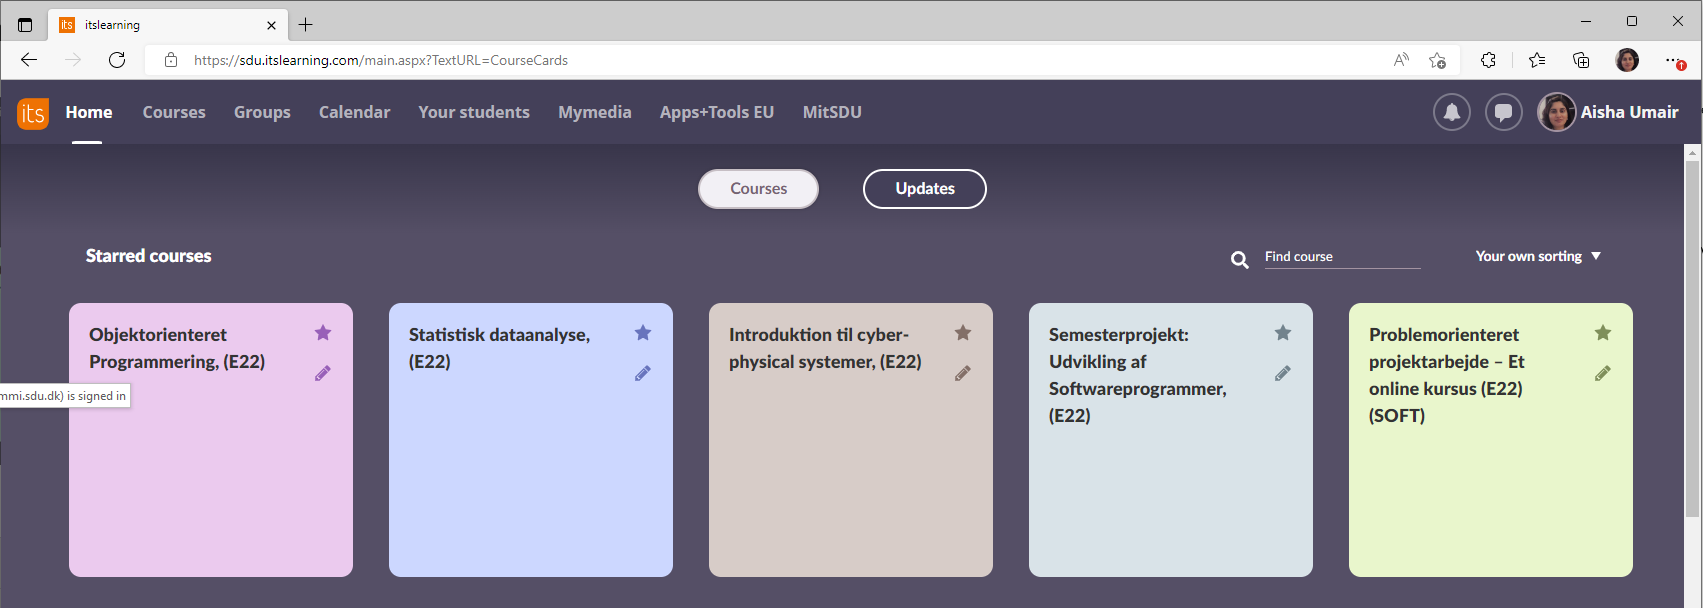
\includegraphics[width=14cm]{figs/itslearning/courses.png}
  \end{center}
  \begin{tikzpicture}[remember picture, overlay]
    \tikzstyle{edge}  = [
      very thick,
      >=stealth,
      draw=red,
    ]
    \node[ellipse, draw=red, very thick, minimum width=10mm, minimum height=6mm] (home) at (7.5mm,49mm) {};
    \node[ellipse, draw=red, very thick, minimum width=14mm, minimum height=8mm] (courses) at (62.5mm,42.5mm) {};
    \node[rectangle, draw=red, very thick, align=left] (note) at (100mm,69mm) {\textcolor{red}{For SE students, it will be}\\\textcolor{red}{Computer Systems course}};
    \coordinate (target) at (77mm,35mm);
    \draw[->, edge] (note) -- (target);
  \end{tikzpicture}
\end{frame}

\subsection{Home Page: Updates (tab)}
\begin{frame}[fragile]
  \frametitle{Home Page: Updates (tab)}
  \vspace{2.2mm}
  \begin{center}
    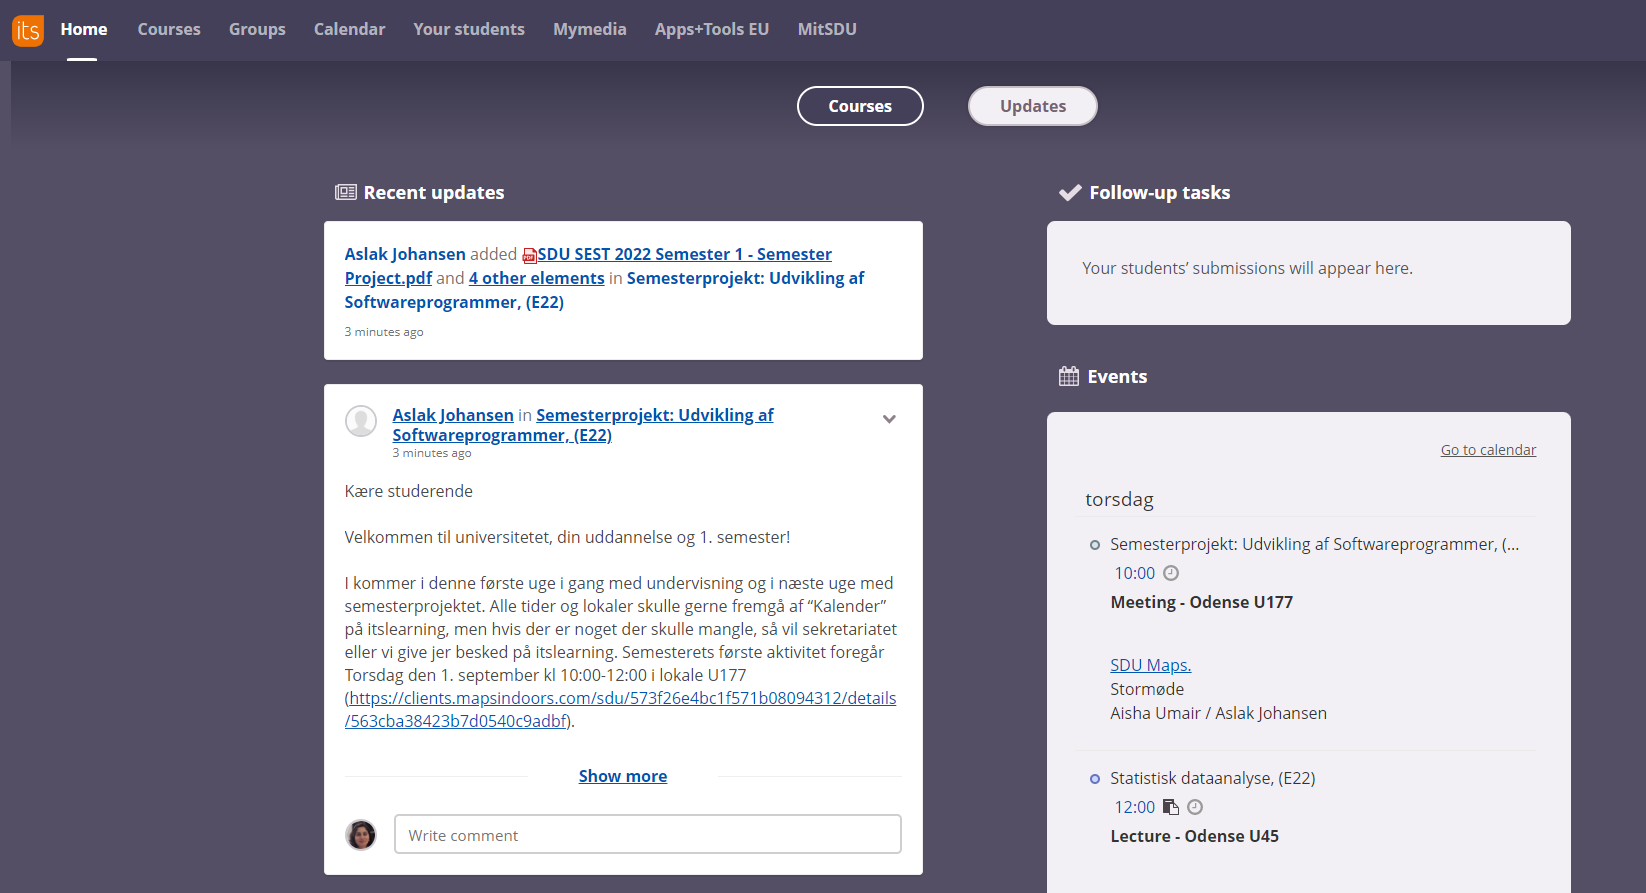
\includegraphics[width=14cm]{figs/itslearning/updates.png}
  \end{center}
  \begin{tikzpicture}[remember picture, overlay]
    \node[ellipse, draw=red, very thick, minimum width=17mm, minimum height=9mm] (courses) at (88mm,73.25mm) {};
  \end{tikzpicture}
\end{frame}

\subsection{Home Page: Courses (tab)}
\begin{frame}[fragile]
  \frametitle{Home Page: Courses (tab)}
  \vspace{9mm}
  \begin{center}
    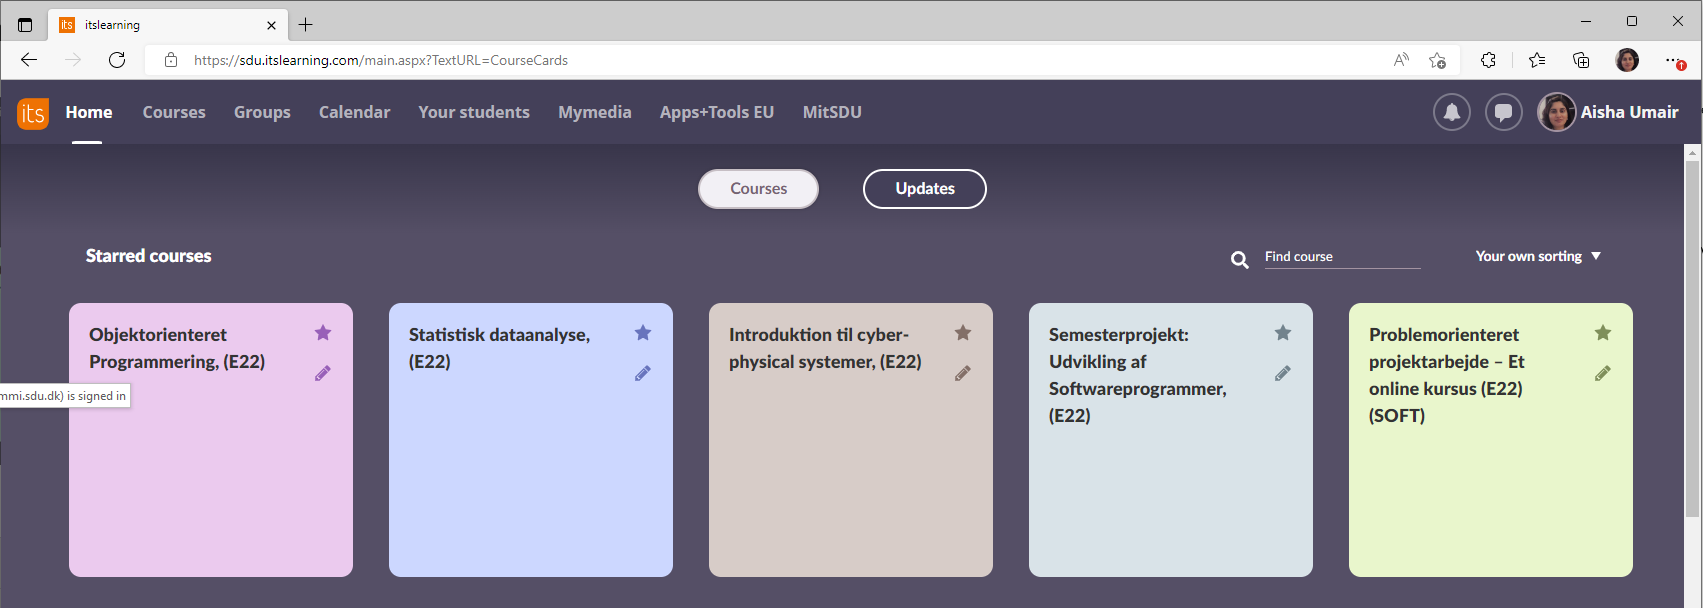
\includegraphics[width=14cm]{figs/itslearning/courses.png}
  \end{center}
  \begin{tikzpicture}[remember picture, overlay]
    \node[rectangle, rounded corners, draw=red, very thick, minimum width=25mm, minimum height=25mm] (highlight) at (96.4mm,21.8mm) {};
  \end{tikzpicture}
\end{frame}

\subsection{Semesterprojekt: Front Page}
\begin{frame}[fragile]
  \frametitle{Semesterprojekt: Front Page}
  \vspace{-1mm}
  \begin{center}
    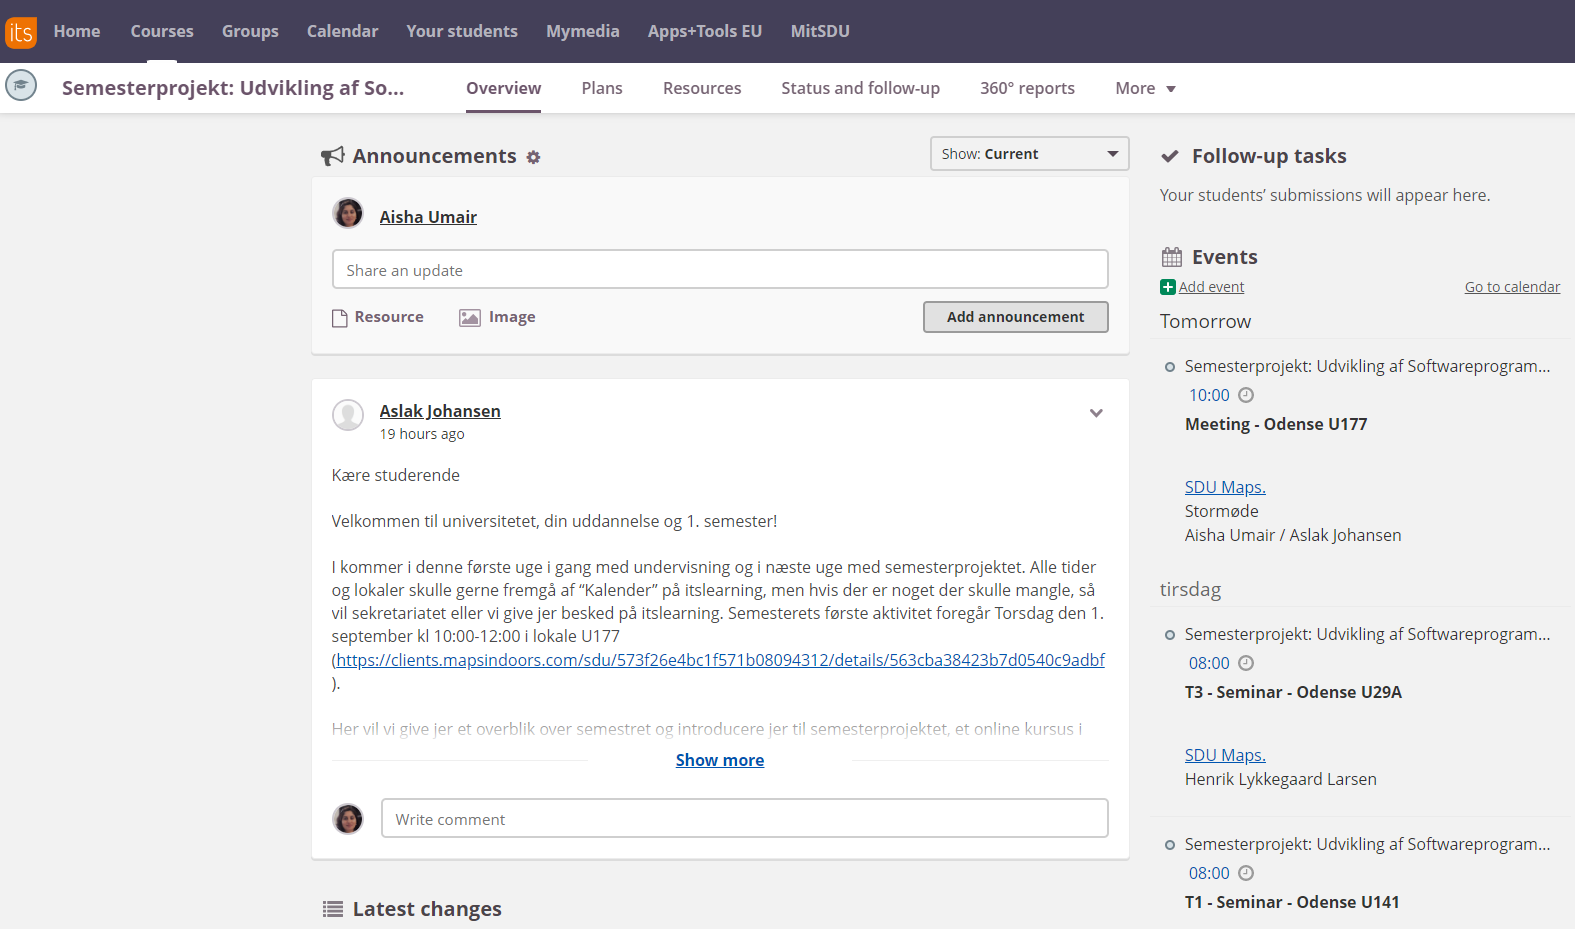
\includegraphics[width=13.4cm]{figs/itslearning/overview.png}
  \end{center}
\end{frame}

\subsection{Plans}
\begin{frame}[fragile]
  \frametitle{Plans}
  \vspace{-3mm}
  \begin{center}
    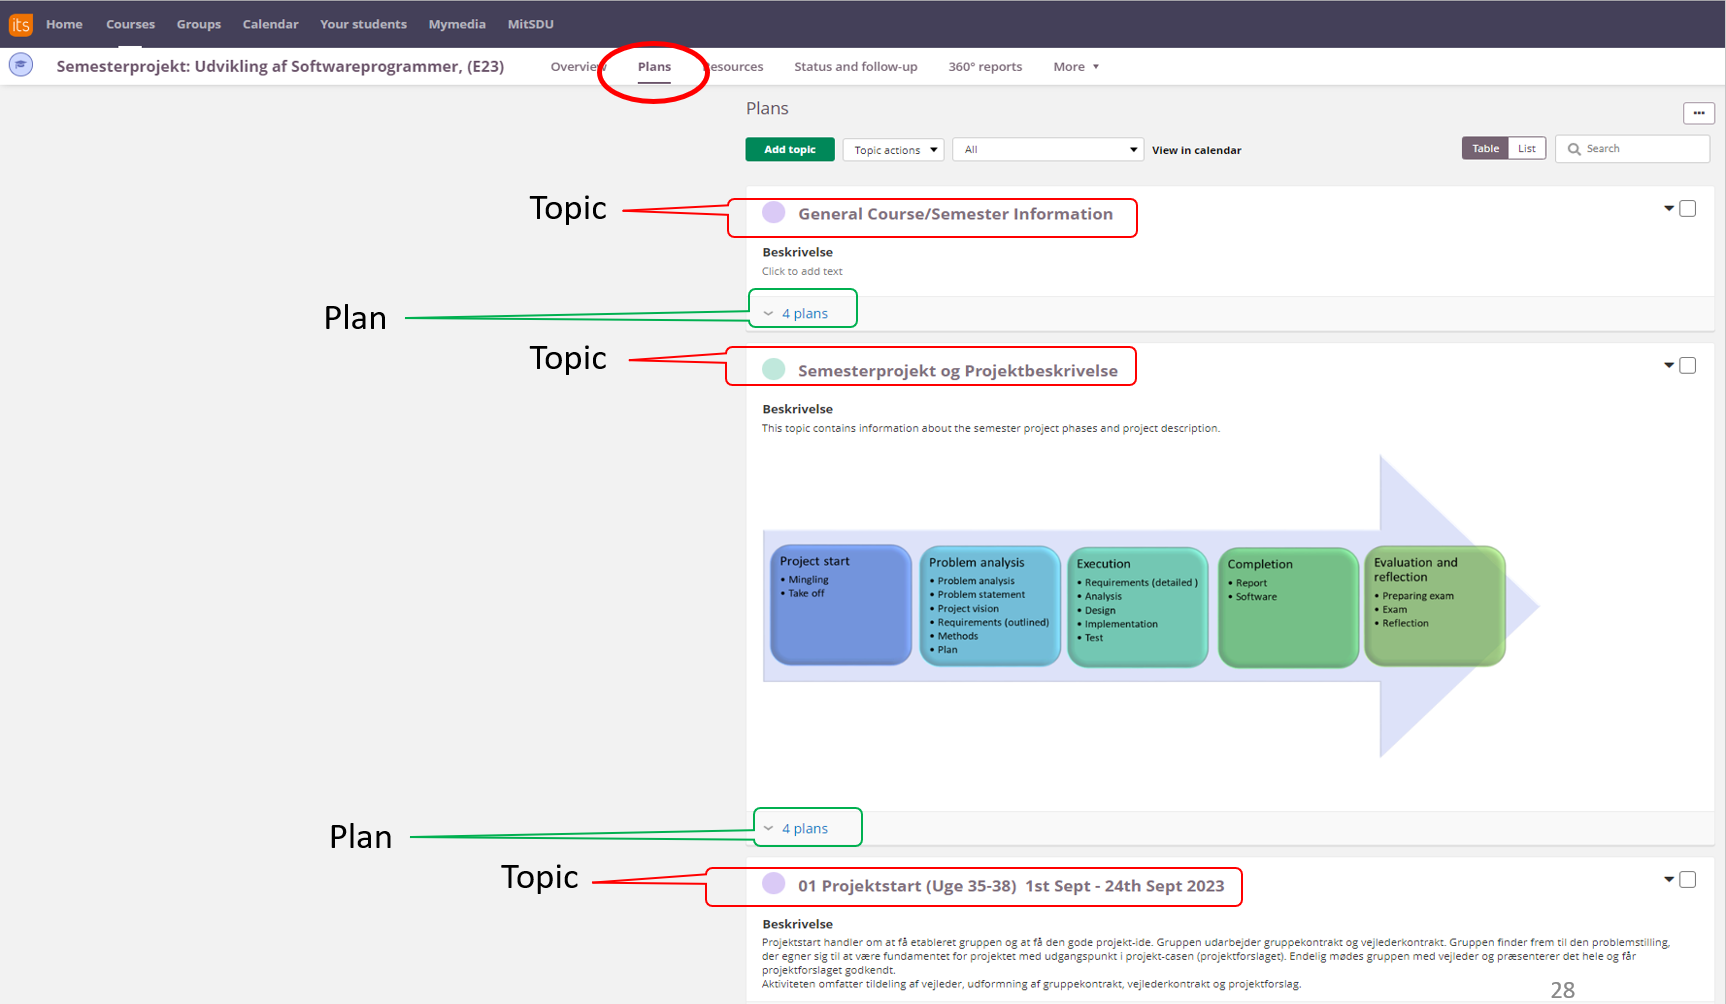
\includegraphics[width=122mm]{figs/itslearning/plans.png}
  \end{center}
  \begin{tikzpicture}[remember picture, overlay]
    \tikzstyle{edge}  = [
      very thick,
      >=stealth,
      draw=red,
    ]
    \node[ellipse, draw=red, very thick, minimum width=7mm, minimum height=5mm] (plans) at (52.75mm,76mm) {};
    
    \node[rectangle, draw=red, very thick, anchor=north west, minimum width=29mm, minimum height=4mm] (topic1) at (47.5mm,66.25mm) {};
    \node[anchor=east] (topic1label) at ([xshift=-1cm] topic1.west) {\textcolor{red}{Topic}};
    \draw[->, edge] (topic1label) -- (topic1);
    
    \node[rectangle, draw=red, very thick, anchor=north west, minimum width=29mm, minimum height=4mm] (topic2) at (47.5mm,58.5mm) {};
    \node[anchor=east] (topic2label) at ([xshift=-1cm] topic2.west) {\textcolor{red}{Topic}};
    \draw[->, edge] (topic2label) -- (topic2);
    
    \node[rectangle, draw=red, very thick, anchor=north west, minimum width=37.5mm, minimum height=4mm] (topic3) at (47.5mm,17.3mm) {};
    \node[anchor=east] (topic3label) at ([xshift=-1cm] topic3.west) {\textcolor{red}{Topic}};
    \draw[->, edge] (topic3label) -- (topic3);
    
    \node[rectangle, draw=green!60!black, very thick, anchor=north west, minimum width=7mm, minimum height=2.5mm] (plan) at (47.5mm,61.7mm) {};
    \node[anchor=west] (planlabel) at ([xshift=3cm] plan.east) {\textcolor{green!60!black}{Plan}};
    \draw[->, edge, draw=green!60!black] (planlabel) -- (plan);
  \end{tikzpicture}
\end{frame}

\subsection{Resources}
\begin{frame}[fragile]
  \frametitle{Resources}
  \vspace{-1.5mm}
  \begin{center}
    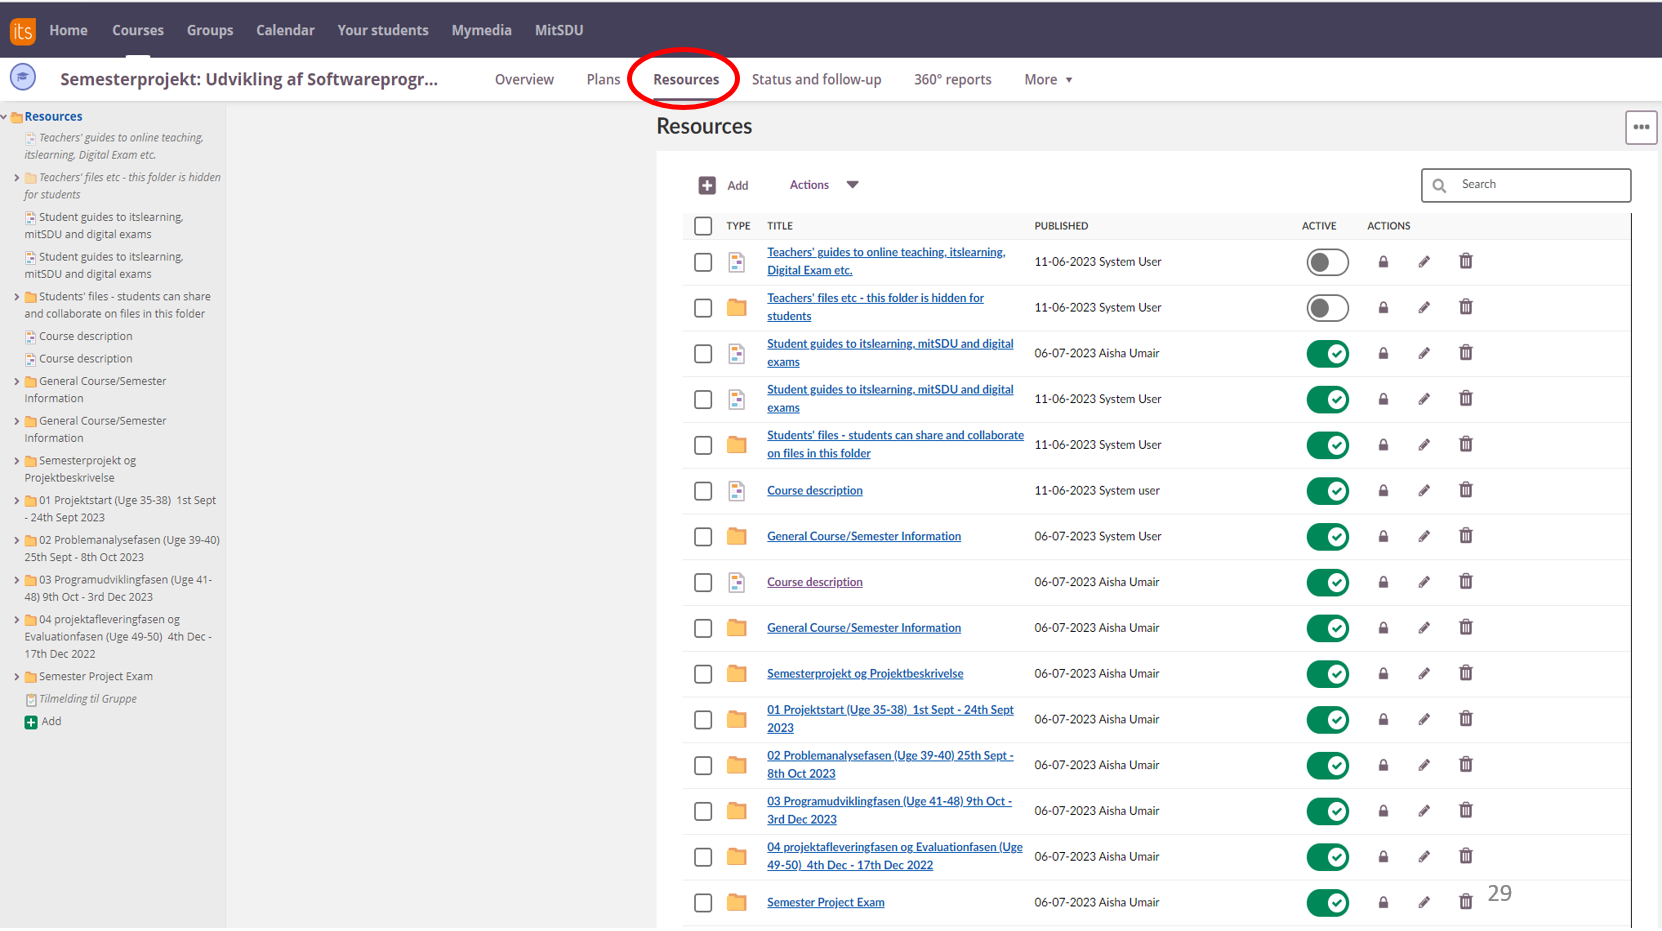
\includegraphics[width=140mm]{figs/itslearning/resources.png}
  \end{center}
  \begin{tikzpicture}[remember picture, overlay]
    \tikzstyle{edge}  = [
      very thick,
      >=stealth,
      draw=red,
    ]
    \node[ellipse, draw=red, very thick, minimum width=9mm, minimum height=5mm] (plans) at (56.5mm,73.2mm) {};
  \end{tikzpicture}
\end{frame}

\subsection{Status and Follow-Up}
\begin{frame}[fragile]
  \frametitle{Status and Follow-Up}
  \vspace{12mm}
  \begin{center}
    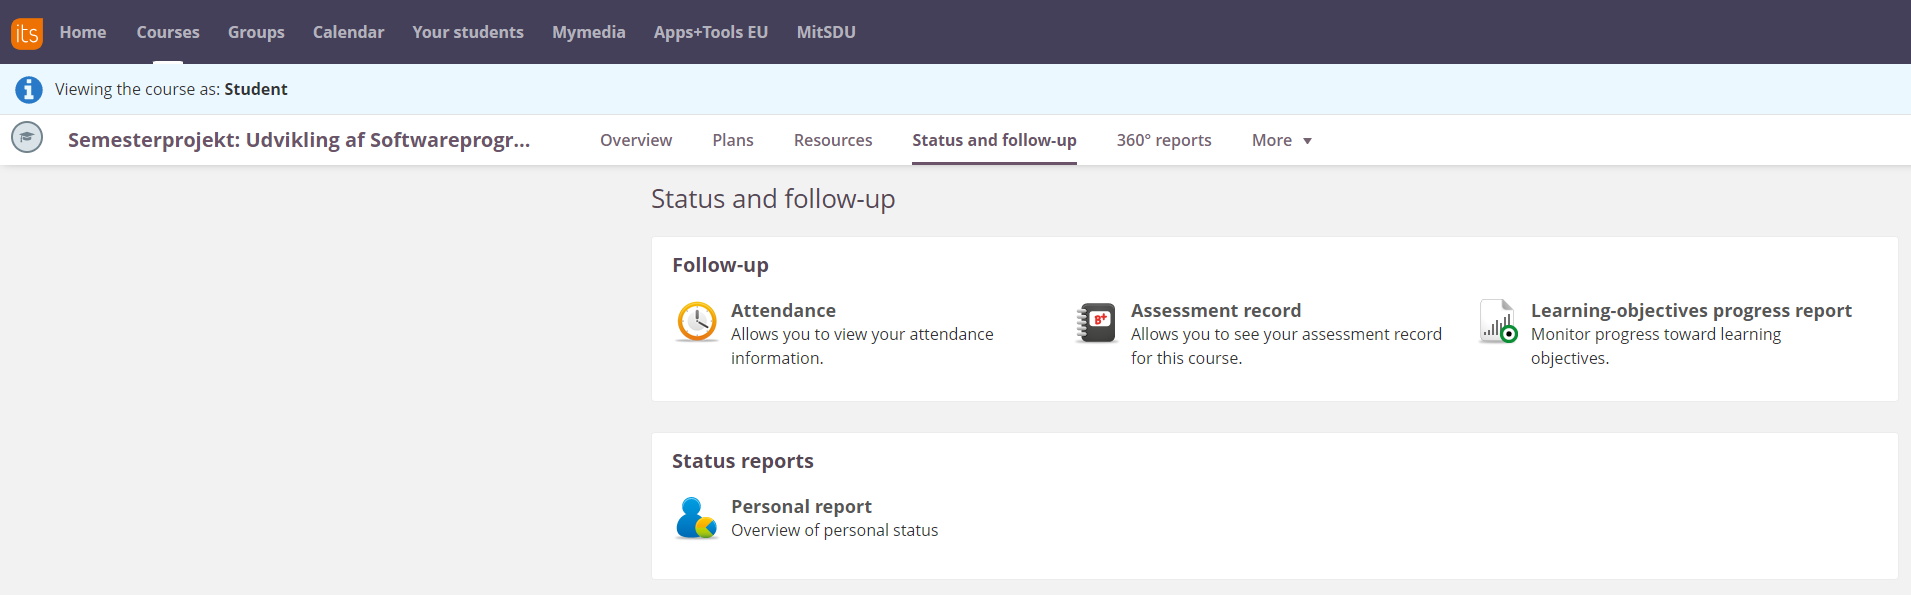
\includegraphics[width=140mm]{figs/itslearning/status-and-followup.png}
  \end{center}
  \begin{tikzpicture}[remember picture, overlay]
    \tikzstyle{edge}  = [
      very thick,
      >=stealth,
      draw=red,
    ]
    \node[ellipse, draw=red, very thick, minimum width=16mm, minimum height=6mm] (plans) at (72.8mm,41.2mm) {};
  \end{tikzpicture}
\end{frame}

\subsection{Semester Projekt: Course Structure}
\begin{frame}[fragile]
  \frametitle{Semester Projekt: Course Structure}
  \vspace{30mm}
  \begin{center}
    Let's visit the website together: \textcolor{blue}{\url{https://sdu.itslearning.com}}
  \end{center}
\end{frame}

%%%%%%%%%%%%%%%%%%%%%%%%%%%%%%%%%%%%%%%%%%%%%%%%%%%%%%%%%%%%%%%
%%%%%%%%%%%%%%%%%%%%%%%%%%%%%%%%%%%%%%%%%%%%%%%%%%%%% ProOnline
\section{ProOnline}
\begin{frame}
  \vspace{25mm}
  \begin{center}
    \Huge{Part 3:\\ProOnline}
  \end{center}
\end{frame}

\subsection{Home Page: Courses (tab)}
\begin{frame}[fragile]
  \frametitle{Home Page: Courses (tab)}
  \vspace{9mm}
  \begin{center}
    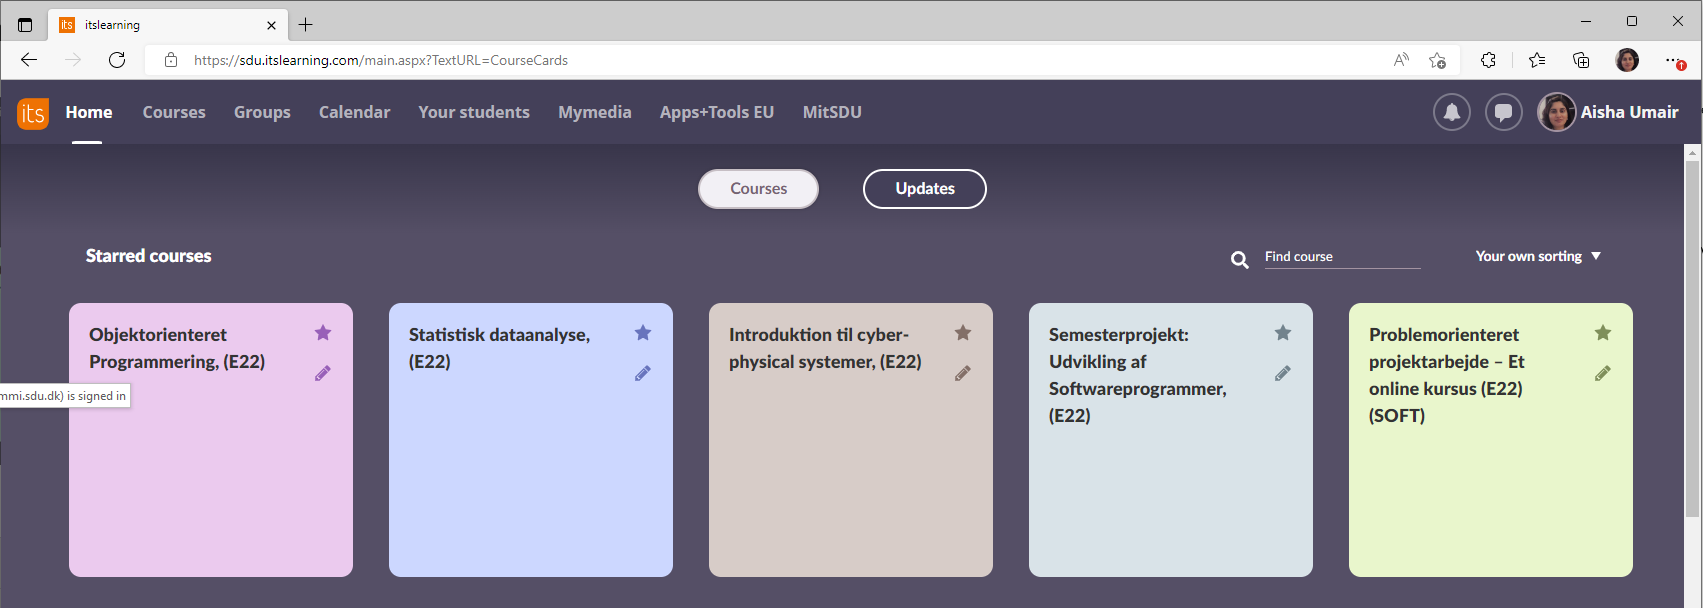
\includegraphics[width=14cm]{figs/itslearning/courses.png}
  \end{center}
  \begin{tikzpicture}[remember picture, overlay]
    \node[rectangle, rounded corners, draw=red, very thick, minimum width=25mm, minimum height=25mm] (highlight) at (122.65mm,21.8mm) {};
  \end{tikzpicture}
\end{frame}

\subsection{Problemorienteret Projektarbejde - et Online Kursus}
\begin{frame}[fragile]
  \frametitle{Problemorienteret Projektarbejde - et Online Kursus}
  \vspace{1mm}
  \begin{itemize}
    \item Støtter den studerende i projektarbejde i forbindelse med studiet.
    \item Giver indsigt og træning inden for problemorienteret projektarbejde,
samarbejde, afrapportering og eksamen.
  \end{itemize}
  
  \begin{tikzpicture}[remember picture, overlay]
    \node[anchor=south east] (image) at (current page.south east) {
      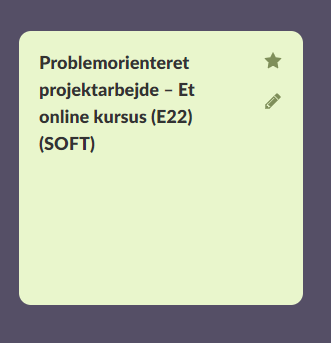
\includegraphics[width=6cm]{figs/itslearning/proonline-box.png}
    };
  \end{tikzpicture}
\end{frame}

\subsection{Problemorienteret Projektarbejde - et Online Kursus}
\begin{frame}[fragile]
  \frametitle{Problemorienteret Projektarbejde - et Online Kursus}
  \vspace{-5mm}
  
\begin{tikzpicture}[remember picture, overlay]
    \newcommand{\spacing}[0]{4mm}
    \newcommand{\xshift}[0]{12mm}
    \newcommand{\yshift}[0]{4mm}
    
    \tikzstyle{box} = [
      draw=black,
      very thick,
      anchor=north west,
      align=center,
      minimum width=42mm,
      minimum height=16mm,
    ]
    \tikzstyle{edge} = [
      ->,
      very thick,
      >=stealth,
    ]
    \tikzstyle{edgeblue} = [
      edge,
      draw=blue,
    ]
    \tikzstyle{edgegreen} = [
      edge,
      draw=green!70!black,
    ]
    \tikzstyle{edgeyellow} = [
      edge,
      draw=yellow!40!brown,
    ]
    \node[box] (1) at (0mm,0mm) {\textbf{01:} Introduktion til\\kurset};
    \node[box] (2) at ([yshift=-\spacing] 1.south west) {\textbf{02:} Projekter på\\Ingeniøruddannelserne};
    \node[box] (3) at ([yshift=-\spacing] 2.south west) {\textbf{03:} Samarbejde};
    \node[box] (4) at ([yshift=-\spacing] 3.south west) {\textbf{04:} Problemorienteret\\projektarbejde};
    \node[box] (8) at ([xshift=\spacing] 1.north east) {\textbf{08:} Præsentation og\\feedback};
    \node[box] (7) at ([yshift=-\spacing] 8.south west) {\textbf{07:} Metoder og plan-\\lægning i projektarbejdet};
    \node[box] (6) at ([yshift=-\spacing] 7.south west) {\textbf{06:} Projektets faglige \\vidensgrundlag};
    \node[box] (5) at ([yshift=-\spacing] 6.south west) {\textbf{05:} Problemanalyse og\\problemformulering};
    \node[box] (9) at ([xshift=\spacing] 8.north east) {\textbf{09:} Projektrapporten};
    \node[box] (10) at ([yshift=-\spacing] 9.south west) {\textbf{10:} Projekteksamen};
    
    \draw[edgeblue]   ([xshift=-\xshift] 1.south) -- ([xshift=-\xshift] 2.north);
    \draw[edgegreen]  ([xshift=0       ] 1.south) -- ([xshift=0       ] 2.north);
    \draw[edgeyellow] ([xshift= \xshift] 1.south) -- ([xshift= \xshift] 2.north);
    
    \draw[edgeblue]   ([xshift=-\xshift] 2.south) -- ([xshift=-\xshift] 3.north);
    \draw[edgegreen]  ([xshift=0       ] 2.south) -- ([xshift=0       ] 3.north);
    \draw[edgeyellow] ([xshift= \xshift] 2.south) -- ([xshift= \xshift] 3.north);
    
    \draw[edgeblue]   ([xshift=-\xshift] 3.south) -- ([xshift=-\xshift] 4.north);
    
    \draw[edgeyellow] (3.south east) -- (5.north west);
    
    \draw[edgegreen]  ([yshift=0       ] 3.east) -- ([yshift=0       ] 6.west);
    
    \draw[edgeblue]   ([yshift=\yshift] 4.east) -- ([yshift=\yshift] 5.west);
    
    \draw[edgeblue]   ([xshift=-\xshift] 5.north) -- ([xshift=-\xshift] 6.south);
    \draw[edgeyellow] ([xshift= \xshift] 5.north) -- ([xshift= \xshift] 6.south);
    
    \draw[edgeblue]   ([xshift=-\xshift] 6.north) -- ([xshift=-\xshift] 7.south);
    \draw[edgegreen]  ([xshift=0       ] 6.north) -- ([xshift=0       ] 7.south);
    \draw[edgeyellow] ([xshift= \xshift] 6.north) -- ([xshift= \xshift] 7.south);
    
    \draw[edgeblue]   ([xshift=-\xshift] 7.north) -- ([xshift=-\xshift] 8.south);
    \draw[edgegreen]  ([xshift=0       ] 7.north) -- ([xshift=0       ] 8.south);
    \draw[edgeyellow] ([xshift= \xshift] 7.north) -- ([xshift= \xshift] 8.south);
    
    \draw[edgeblue]   ([yshift= \yshift] 8.east) -- ([yshift= \yshift] 9.west);
    \draw[edgegreen]  ([yshift=0       ] 8.east) -- ([yshift=0       ] 9.west);
    \draw[edgeyellow] ([yshift=-\yshift] 8.east) -- ([yshift=-\yshift] 9.west);
    
    \draw[edgeblue]   ([xshift=-\xshift] 9.south) -- ([xshift=-\xshift] 10.north);
    \draw[edgegreen]  ([xshift=0       ] 9.south) -- ([xshift=0       ] 10.north);
    \draw[edgeyellow] ([xshift= \xshift] 9.south) -- ([xshift= \xshift] 10.north);
  \end{tikzpicture}
\end{frame}

\subsection{Problemorienteret Projektarbejde - et Online Kursus}
\begin{frame}[fragile]
  \frametitle{Problemorienteret Projektarbejde - et Online Kursus}
  \vspace{-2mm}
  \begin{center}
    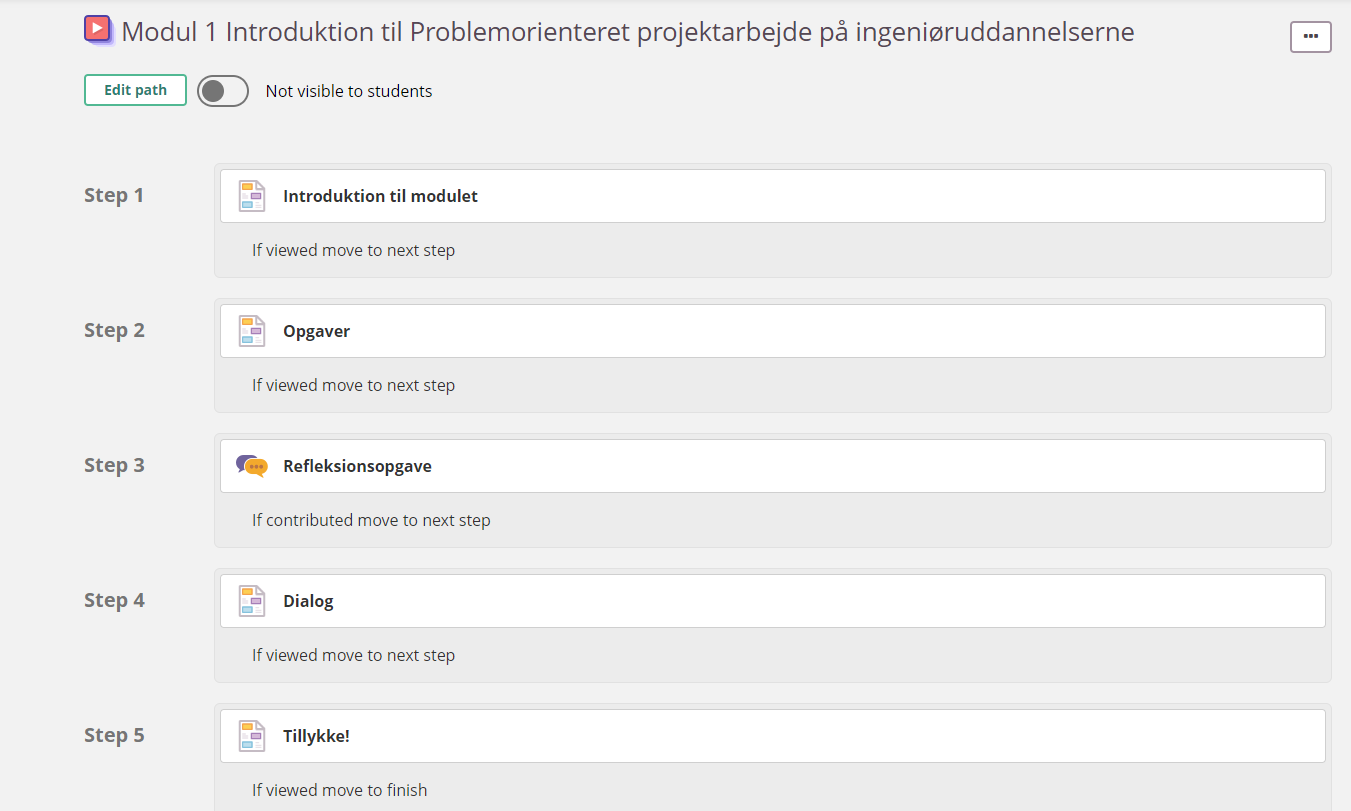
\includegraphics[width=134mm]{figs/itslearning/module1.png}
  \end{center}
\end{frame}

\subsection{Demo}
\begin{frame}[fragile]
  \frametitle{Demo}
  \vspace{30mm}
  \begin{center}
    Lad os kigge på kurset \ldots
  \end{center}
\end{frame}

\subsection{Næste Skridt}
\begin{frame}[fragile]
  \frametitle{Næste Skridt}
  \vspace{1mm}
  Se semesterplanen!
  
  \begin{longtable}{|r|l|p{.4\textwidth}|l|p{.2\textwidth}|}
  \hline
  \emph{Uge} & \emph{Aktivitet} & \emph{Beskrivelse} & \emph{Date} & \emph{Semesterteam} \\
  \hline
  36 & ProOnline & \begin{itemize}

  \item 01 Introduktion til online kursus i problemorienteret projektarbejde

  \item 02 Projekter på ingeniøruddannelserne

\end{itemize} & Sep 4 &  \\
  \hline
  36 & Projekt & \textbf{Vejledningsseminar i klasserne:} Projektstart & Sep 5 & Vejlederteam: briefing \\
  \hline
  36 & ProOnline & \begin{itemize}

  \item 03 Samarbejde

\end{itemize} & Sep 8 &  \\
  \hline
\end{longtable}

\end{frame}

\subsection{Skema}
\begin{frame}[fragile]
  \frametitle{Skema}
  \vspace{0mm}
  
\begin{tikzpicture}[remember picture, overlay]
    % variables
    \newcommand{\blockw}[0]{28mm}
    \newcommand{\blockh}[0]{14mm}
    
    % styles
    \tikzstyle{day}  = [
      anchor=south,
    ]
    \tikzstyle{block}  = [
      anchor=north west,
      minimum width=\blockw,
      minimum height=\blockh,
      draw,
    ]
    \tikzstyle{time}  = [
      anchor=east,
    ]
    \tikzstyle{lecture}  = [
      anchor=north west,
      minimum width=\blockw,
      minimum height=\blockh,
      draw=purple,
      fill=purple!50,
      align=center,
    ]
    \tikzstyle{exercise}  = [
      anchor=north west,
      minimum width=\blockw,
      minimum height=\blockh,
      draw=teal,
      fill=teal!50,
      align=center,
    ]
    \tikzstyle{project}  = [
      anchor=north west,
      minimum width=\blockw,
      minimum height=5*\blockh,
      draw=black,
      fill=black!25,
      align=center,
    ]
    
    \coordinate (origo)     at (2mm,0mm);
    
    % coordinates: days
    \coordinate (monday)    at ([xshift=0*\blockw] origo);
    \coordinate (tuesday)   at ([xshift=1*\blockw] origo);
    \coordinate (wednesday) at ([xshift=2*\blockw] origo);
    \coordinate (thursday)  at ([xshift=3*\blockw] origo);
    \coordinate (friday)    at ([xshift=4*\blockw] origo);
    
    % coordinates: blocks
    \coordinate (monday08)  at ([yshift= 0*\blockh] monday);
    \coordinate (monday10)  at ([yshift=-1*\blockh] monday);
    \coordinate (monday12)  at ([yshift=-2*\blockh] monday);
    \coordinate (monday14)  at ([yshift=-3*\blockh] monday);
    \coordinate (monday16)  at ([yshift=-4*\blockh] monday);
    \coordinate (monday18)  at ([yshift=-5*\blockh] monday);
    \coordinate (tuesday08)  at ([yshift= 0*\blockh] tuesday);
    \coordinate (tuesday10)  at ([yshift=-1*\blockh] tuesday);
    \coordinate (tuesday12)  at ([yshift=-2*\blockh] tuesday);
    \coordinate (tuesday14)  at ([yshift=-3*\blockh] tuesday);
    \coordinate (tuesday16)  at ([yshift=-4*\blockh] tuesday);
    \coordinate (wednesday08)  at ([yshift= 0*\blockh] wednesday);
    \coordinate (wednesday10)  at ([yshift=-1*\blockh] wednesday);
    \coordinate (wednesday12)  at ([yshift=-2*\blockh] wednesday);
    \coordinate (wednesday14)  at ([yshift=-3*\blockh] wednesday);
    \coordinate (wednesday16)  at ([yshift=-4*\blockh] wednesday);
    \coordinate (thursday08)  at ([yshift= 0*\blockh] thursday);
    \coordinate (thursday10)  at ([yshift=-1*\blockh] thursday);
    \coordinate (thursday12)  at ([yshift=-2*\blockh] thursday);
    \coordinate (thursday14)  at ([yshift=-3*\blockh] thursday);
    \coordinate (thursday16)  at ([yshift=-4*\blockh] thursday);
    \coordinate (friday08)  at ([yshift= 0*\blockh] friday);
    \coordinate (friday10)  at ([yshift=-1*\blockh] friday);
    \coordinate (friday12)  at ([yshift=-2*\blockh] friday);
    \coordinate (friday14)  at ([yshift=-3*\blockh] friday);
    \coordinate (friday16)  at ([yshift=-4*\blockh] friday);
    
    % blocks
    \node[block] () at (monday08) {};
    \node[block] () at (monday10) {};
    \node[block] () at (monday12) {};
    \node[block] () at (monday14) {};
    \node[block] () at (monday16) {};
    \node[block] () at (tuesday08) {};
    \node[block] () at (tuesday10) {};
    \node[block] () at (tuesday12) {};
    \node[block] () at (tuesday14) {};
    \node[block] () at (tuesday16) {};
    \node[block] () at (wednesday08) {};
    \node[block] () at (wednesday10) {};
    \node[block] () at (wednesday12) {};
    \node[block] () at (wednesday14) {};
    \node[block] () at (wednesday16) {};
    \node[block] () at (thursday08) {};
    \node[block] () at (thursday10) {};
    \node[block] () at (thursday12) {};
    \node[block] () at (thursday14) {};
    \node[block] () at (thursday16) {};
    \node[block] () at (friday08) {};
    \node[block] () at (friday10) {};
    \node[block] () at (friday12) {};
    \node[block] () at (friday14) {};
    \node[block] () at (friday16) {};
    
    % schedule
    \node[lecture]  () at (monday10) {\textbf{OOP} \\ \scriptsize Forelæsning i U45};
    \node[exercise] () at (monday12) {\textbf{OOP} \\ \scriptsize Øvelser};
    \node[project]  () at (tuesday08) {\textbf{Project}};
    \node[lecture]  () at (wednesday12) {\textbf{OOP} \\ \scriptsize Forelæsning i U45};
    \node[exercise] () at (wednesday14) {\textbf{OOP} \\ \scriptsize Øvelser};
    \node[lecture]  () at (thursday12) {\textbf{SDA} \\ \scriptsize Forelæsning i U45};
    \node[exercise] () at (thursday14) {\textbf{SDA} \\ \scriptsize Øvelser};
    \node[lecture]  () at (friday10) {\textbf{COS/CPS} \\ \scriptsize Forelæsning i U45};
    \node[exercise] () at (friday12) {\textbf{COS/CPS} \\ \scriptsize Øvelser};
    
    % time
    \node[time] () at (monday08) {8};
    \node[time] () at (monday10) {10};
    \node[time] () at (monday12) {12};
    \node[time] () at (monday14) {14};
    \node[time] () at (monday16) {16};
    \node[time] () at (monday18) {18};
    
    % days
    \node[day] () at ([xshift=\blockw/2] monday)    {Mandag};
    \node[day] () at ([xshift=\blockw/2] tuesday)   {Tirsdag};
    \node[day] () at ([xshift=\blockw/2] wednesday) {Onsdag};
    \node[day] () at ([xshift=\blockw/2] thursday)  {Torsdag};
    \node[day] () at ([xshift=\blockw/2] friday)    {Fridag};
  \end{tikzpicture}
\end{frame}

\subsection{How to Uni}
\begin{frame}[fragile]
  \frametitle{How to Uni}
  \vspace{30mm}
  \begin{center}
    Husk at gennemføre 1. semesterprøven før deadline (7th September)
  \end{center}
\end{frame}

%%%%%%%%%%%%%%%%%%%%%%%%%%%%%%%%%%%%%%%%%%%%%%%%%%%%%%%%%%%%%%%
%%%%%%%%%%%%%%%%%%%%%%%%%%%%%%%%%%%%%%%%%%%%%%%%%%%%% Thank You
\section{Thank You}
\begin{frame}
  \vspace{25mm}
  \begin{center}
    \Huge{Thank You\\Wish you Good Luck \smiley{}}
  \end{center}
\end{frame}

\end{document}
